\documentclass[12pt]{report}
%\documentclass[12pt]{article}
\usepackage{tabularx,graphicx,layout}
\usepackage{hyperref}
\usepackage{blindtext}
\usepackage[utf8]{inputenc}
\usepackage{enumitem}
\usepackage{pifont}
\usepackage{xcolor}
\usepackage{version}
\setcounter{secnumdepth}{5}
\setcounter{tocdepth}{5}

\begin{document}
\title{Experiment Safety Assessment Document (ESAD) \\ 
for the Hall B CLAS12 Run Group D}
\date{Updated on \today\ for Run Group D (RG-D)}
%
% LaTeX Version 12 GeV ESAD 
%
%
\maketitle
\tableofcontents

\chapter{Introduction}

This ESAD document describes the identified hazards of the experiment and the measures 
taken to eliminate, control, or mitigate them. This document is part of the CEBAF 
experiment review process as defined in
\href{http://www.jlab.org/ehs/ehsmanual/manual/3120.html}{Chapter 3120} of the Jefferson 
Lab EHS\&Q manual, and will start by describing general types of hazards that might be 
present in any of the JLab experimental halls.  The document then addresses the hazards 
associated with subsystems of the equipment in Experimental Hall~B and their mitigation.  
Responsible personnel for each item are also noted. In case of life threatening emergencies 
call 911 and then notify the guard house at x5822 so that the guards can help the 
responders.  This document does not attempt to describe the function or operation of the 
various subsystems. Such information can be found in the individual subsystem Operations 
Manuals.

\chapter{General Hazards}

\section{Radiation}
	
CEBAF's high intensity and high energy electron beam is a potentially lethal direct 
radiation source. It can also create radioactive materials that are hazardous even after 
the beam has been turned off. There are many redundant measures aimed at preventing 
accidental exposure to personnel by the beam or exposure to beam-associated radiation 
sources that are in place at JLab. The training and mitigation procedures are handled 
through the JLab Radiation Control Department (RadCon). RadCon can be contacted as follows: 
For routine support and surveys, or for emergencies after-hours, call the RadCon cell phone 
at 876-1743. For escalation of effort or for emergencies, the RadCon manager (Keith Welch) 
can be reached as follows: Office: 757-269-7212.

Radiation damage to materials and electronics is mainly determined by the neutron 
dose (photon dose typically causes parity errors and is easier to shield against). 
Commercial-off-the-shelf (COTS) electronics is typically robust up to neutron doses of 
about $10^{13}$~n/cm$^2$. If the experimental equipment dose as calculated in the RSAD 
is beyond this damage threshold, the experiment needs to add an appendix on ``Evaluation 
of potential radiation damage" in the experiment-specific ESAD. There, the radiation 
damage dose, potential impact to equipment located in areas above this damage threshold, 
as well as the mitigating measures to be taken should be described.

\section{Fire}

Each of the experimental halls contains numerous combustible materials and flammable gases. 
In addition, they contain potential ignition sources, such as electrical wiring and equipment. 
General fire hazards and procedures for dealing with these are covered by JLab emergency 
management procedures. The JLab fire protection manager (Tim Minga) can be contacted at 
757-269-731, Cell: 757-371-16870.

\section{Electrical Systems}

Hazards associated with electrical systems are the most common risk in the experimental 
halls. Almost every subsystem requires AC and/or DC power. Due to the high current and/or 
high voltage requirements of many of these subsystems, they and their power supplies are 
potentially lethal electrical sources. In the case of superconducting magnets the stored 
energy is so large that an uncontrolled electrical discharge can be lethal for a period of 
time even after the actual power source has been turned off. Anyone working on electrical 
power in the experimental halls must comply with 
\href{http://www.jlab.org/ehs/ehsmanual/manual/6200.html}{Chapter 6200} of the Jefferson Lab 
EHS\&Q manual and must obtain approval of one of the responsible personnel. The JLab 
electrical safety point-of-contact (Chad Bailey) can be reached at 757-269-7052.

\section{Mechanical Systems}

There exist a variety of mechanical hazards in all experimental halls at JLab. Numerous 
electro-mechanical subsystems are massive enough to produce potential fall and/or crush 
hazards.  In addition, heavy objects are routinely moved around within the experimental 
halls during reconfigurations for specific experiments. 

Use of ladders and scaffolding must comply with 
\href{http://www.jlab.org/ehs/ehsmanual/manual/6132.html}{Chapter 6132} of the Jefferson 
Lab EHS\&Q manual. Use of cranes, hoists, lifts, etc. must comply with
\href{http://www.jlab.org/ehs/ehsmanual/manual/6141.html}{Chapter 6141} of the Jefferson
Lab EHS\&Q manual. Use of personal protective equipment to mitigate mechanical hazards, 
such as hard hats, safety harnesses, and safety shoes, are mandatory when deemed necessary.
The JLab technical point-of-contact (Jennifer Williams) can be contacted at 757-269-7882.

\section{Strong Magnetic Fields}

Powerful magnets exist in all JLab experimental halls. Metal objects may be attracted 
by the magnet fringe field and become airborne, possibly injuring body parts or striking 
fragile components, resulting in a cascading hazard condition. Cardiac pacemakers or other 
electronic medical devices may no longer function properly in the presence of magnetic 
fields. Metallic medical implants (non-electronic) may be adversely affected by magnetic 
fields. Loss of information from magnetic data storage devices such as tapes, disks, and 
credit cards may also occur. Contact Jennifer Williams at 757-269-7882, in case of questions
or concerns.

\section{Cryogenic Fluids and Oxygen Deficiency \\Hazard}

Cryogenic fluids and gases are commonly used in the experimental halls at JLab. When 
released in an uncontrolled manner these can result in explosion, fire, cryogenic burns, 
and the displacement of air, resulting in an oxygen deficiency hazard (ODH) condition. 
The hazard level and associated mitigation are dependent on the subsystem and cryogenic 
fluid. However, they are mostly associated with cryogenic superconducting magnets and 
cryogenic target systems. Flammable cryogenic gases used in the experimental halls 
include hydrogen and deuterium, which are colorless, odorless gases and, hence, not easily 
detected by human senses. Hydrogen air mixtures are flammable over a large range of relative 
concentrations from 4\% to 75\% H$_2$ by volume. Non-flammable cryogenic gases typically 
used include He and nitrogen. Contact Jennifer Williams at 757-269-7882 in case of questions or concerns.

\section{Vacuum and Pressure Vessels}

Vacuum and/or pressure vessels are commonly used in the experimental halls. Many 
of these have thin aluminum or Kevlar/Mylar windows that are close to the entrance 
and/or exit of the vessels or beampipes. These windows burst if punctured accidentally 
or can fail if significant over-pressure were to exist. Injury is possible if a failure 
were to occur near an individual. All work on vacuum windows in the experimental halls 
must occur under the supervision of appropriately trained JLab personnel. Specifically, 
the scattering chamber and beamline exit windows must always be leak checked before 
service. Contact Tim Michalski 757-269-6523 for vacuum and pressure vessel issues.

\section{Hazardous Materials}

Hazardous materials in the form of solids, liquids, and gases that may harm people or 
property exist in the JLab experimental halls. The most common of these materials 
include lead, beryllium compounds, and various toxic and corrosive chemicals. Material 
Safety Data Sheets (MSDS) for hazardous materials in use in the experimental hall are 
available from the hall Safety Wardens. These are being replaced by the new standard
Safety Data Sheets (SDS) as they become available in compliance with the new OSHA 
standards. Handling of these materials must follow the guidelines of the EHS\&Q manual. 
Machining of lead or beryllium, which are highly toxic in powdered form, requires prior 
approval of the EHS\&Q staff. Lead Worker training is required in order to handle lead in 
the experiment halls. In case of questions or concerns, the JLab hazardous materials 
specialist (Scott Conley) can be contacted at 757-269-7308.

\section{Lasers}

High power lasers are often used in the experimental areas for various purposes. Improperly 
used lasers are potentially dangerous. Exposure to laser beams at sufficient power levels 
may cause thermal and photochemical injury to the eye, resulting in retina burns and 
blindness. Skin exposure to laser beams may induce pigmentation, accelerated aging, or 
severe skin burns. Laser beams may also ignite combustible materials creating a fire hazard. 
At JLab, lasers with power higher than 5~mW (Class IIIB) can only be operated in a controlled 
environment with proper eye protection and engineering controls designed and approved for the 
specific laser system. Each specific laser system shall be operated under the supervision of 
a Laser System Supervisor (LSS) following the Laser Operating Safety Procedure (LOSP) for 
that system approved by the Laboratory Laser Safety Officer (LSO). The LSO (Jennifer Williams) can 
be reached at 757-269-7556.
%
% details for each of the Halls
%
\chapter{Hall~B-Specific Equipment}

\section{Overview}

The Hall~B subsystems included in this chapter are considered part of the End-station 
Experimental Equipment for the Run-Group M run. Many of these subsystems impose 
similar hazards, such as those induced by magnets and magnet power supplies, high voltage 
systems, cryogenic systems, and vacuum systems. Note that a specific subsystem may have 
many unique hazards associated with it. For each major system, the hazards, mitigations, 
and responsible personnel are noted.

The material in this chapter is a subset of the material in the Hall~B subsystem Operations 
Manuals and is only intended to familiarize people with the hazards and responsible personnel 
for these systems. In no way should it be taken as sufficient information to use or operate 
this equipment.

\section{Detector Checkout System}

The Hall~B equipment readiness for the beam run will be done using the CEBAF Hot Checkout 
system (HCO)~\cite{hco}. Each detector system has its own subsystems and items that have 
to be checked and signed off by the appropriate groups. The systems that have been checked 
and signed as ready for beam will be indicated by a green ``thumbs up". Subsystems that are 
still waiting for readiness check-up and approval will be indicated with red crosses. 

In order to make sure that hall equipment that should be tied into the machine Fast Shutdown 
(FSD) system has been properly checked, the hall Work Coordinator must be notified by e-mail 
prior to the end of each installation period by the system owner that the checks have been 
performed in conjunction with accelerator operations (i.e. checking that the equipment's 
signals will in fact cause an FSD). These notifications will be noted in the Work Coordinator's 
final checklist as having been done. System owners are responsible for notifying the Work 
Coordinator that their system has an FSD tie-in so it can be added to the checklist.

The hall will get permission to run beam only after all systems tied to the delivery of the 
beam to the designated destination are signed off. At that point the main Hall~B system will 
indicate ``Ready" in the HCO tree.

\section{Beamline}

The control and measurement equipment along the Hall~B beamline consists of various 
elements necessary to transport the beam with the required specifications onto the 
production target and the beam dump, and simultaneously to measure the properties of 
the beam relevant to the successful implementation of the physics program in Hall~B. 

The beamline in the hall provides the interface between the CEBAF accelerator and the 
experimental hall. All work on the beamline must be coordinated with both the Physics 
Division and the Accelerator Division in order to ensure safe and reliable transport of 
the electron beam to the dump. The Accelerator Division has the primary responsibility 
of delivering the electron beam to the experimental target and designated dumps.

\subsection{Hazards} 

Along the beamline various hazards can be found. These include radiation areas, vacuum 
windows, high voltage, and magnetic fields.

\subsection{Mitigations}

All magnets (dipoles, quadrupoles, sextupoles, beam correctors) and beam diagnostic devices 
(BPMs, scanners, beam loss monitors, viewers) necessary to transport and monitor the beam 
are controlled by the Machine Control Center (MCC) and/or Hall~B personnel through EPICS 
\cite{epics}. The detailed operational procedures for the Hall~B beamline are essentially 
the same as those for the CEBAF machine and beamline.

Personnel who need to work near or around the beamline should keep in mind the potential 
hazards:
\begin{itemize}
\item Radiation ``Hot Spots" - marked by an ARM or RadCon personnel,
\item Vacuum in beamline elements and other vessels,
\item Thin-windowed vacuum enclosures (e.g. the scattering chamber),
\item Electric power hazards in the vicinity of magnets, and 
\item Conventional hazards (fall hazard, crane hazard, etc.). 
\end{itemize} 

These hazards are noted by signs and the most hazardous areas along the beamline are 
roped off to restrict access when operational (e.g. around the magnets). Signs are posted 
by RadCon for any hot spots. Surveys of the beamline and surrounding areas will be 
performed before any work is done in these areas. The connection of leads to magnets have 
plastic covers for electrical safety. Any work around the magnets will require 
de-energizing the magnets. Energized magnets are noted by red flashing beacons. Any work 
on the magnets requires the ``Lock and Tag" procedures~\cite{ESH}.  

Additional safety information can be obtained from the following documents:
\begin{itemize}[label=$\circ$]

\item ES\&H Manual~\cite{ESH} 

\item PSS description document~\cite{pss}

\item Accelerator Operations Directive~\cite{ops}

\end{itemize} 

\subsection{Responsible Personnel}

The beamline requires both Accelerator and Physics Division personnel to maintain and 
operate. It is very important that both groups stay in contact with each other to 
coordinate any work on the Hall~B beamline. 

\begin{table}[!ht]
\centering
\begin{tabular}{|c|c|c|c|c|} \hline
 Name&Dept.&Phone&email&Comments \\ \hline
Expert on call& &(757)-303-3996&& 1st contact \\ \hline
E. Pasyuk  & Hall~B&x6020&\href{mailto:pasyuk@jlab.org}{\nolinkurl{pasyuk@jlab.org}}&2nd contact \\ \hline
M. Tiefenback & Accel.&x7430&\href{mailto:tiefen@jlab.org}{\nolinkurl{tiefen@jlab.org}}& beamline optics\\ \hline
K. Price      & Accel.&x7067&\href{mailto:kprice@jlab.org}{\nolinkurl{kprice@jlab.org}}&Contact to OPS \\ \hline
\end{tabular}
\caption{Responsible personnel for the Hall B beamline.} 
\label{tb:beam}
\end{table}

\section{Vacuum System}

The Hall~B vacuum system consists of three segments: the beam transport line to the 
experimental target, consisting of 1.5~in to 2.5~in diameter beampipes, the Hall~B 
target vacuum chamber, and the vacuum beamline to the Hall~B electron dump consisting of 
2~in to 6~in diameter beampipes. For all experiments the first two segments are 
interconnected. There is a 1~in diameter, 2-mil-thick aluminum window on the exit of the 
target vacuum chamber and a 2~in diameter, 2-mil-thick window on the entrance of the 
vacuum beamline of the downstream segment. The first part of the CLAS12 Commissioning run 
will use solid targets. In this case all three segments are connected, and instead of the 
target vacuum chamber, a 2~in diameter beampipe will be used. The vacuum spaces can be 
isolated from one another via vacuum valves and the vacuum level can be monitored 
independently using cold cathode gauges. The vacuum in the system is provided by a set of 
roughing, turbo, and ion pumps, and is maintained at a level of better than 
$10^{-5}$~Torr. 

\subsection{Hazards} 

Hazards associated with the vacuum system are due to rapid decompression in case of a window 
failure. Loud noises can cause hearing loss. 

\subsection{Mitigations}

All personnel working in the vicinity of the entrance and exit windows are required to wear 
hearing protection. Warning signs must be posted in that area. In addition, all vacuum vessels 
and piping are designed as pressure vessels.   

\subsection{Responsible Personnel}

The vacuum system will be maintained by the Hall~B Engineering Group.  

\begin{table}[!htb]
\centering
\begin{tabular}{|c|c|c|c|c|} \hline
Name&Dept.&Phone&email&Comments \\ \hline
Engineering on call & Hall~B& (757)-748-5048&& 1st contact  \\ \hline
D. Insley & Hall~B&(757) 897-9060&\href{mailto:dinsley@jlab.org}{\nolinkurl{dinsley@jlab.org}}  &2nd contact \\ \hline
 \end{tabular}
\caption{Personnel responsible for the Hall~B vacuum system.} 
\label{tb:vacuum}
\end{table}



\section{Target System}

The target system used for RG-D is the Hall B cryo target.~This target system has just been assembled and will be used first by RG-D experiments.~RG-D will use the following targets inside the Hall B cryo target system:

\begin{itemize}
\item	Liquid:
   \begin{itemize}
	\item	Hydrogen
	\item	Deuterium
    \end{itemize}
\item		Solid
   \begin{itemize}
	\item	Carbon
	\item	Copper
	\item	Tin
   \end{itemize}
\end{itemize}

The target configuration includes a 5 cm long liquid cell for Hydrogen or Deuterium (LD2), plus a solid target flag system, as shown in Fig.~\ref{fig:rgd-target} below. The flag system holds 2 carbon targets in series or a copper and a tin target in series.  The flag system is mounted in series with the liquid cell. The flag system can be remotely operated to put the carbon targets in the beam, no solid targets in the beam, or the copper and tin targets in the beam.

\begin{figure}\centering
  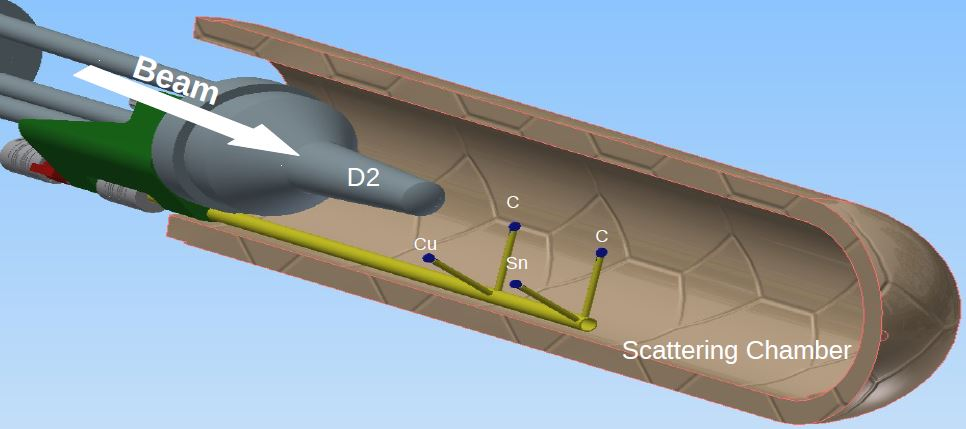
\includegraphics[width=\textwidth]{pics/rgd-target.jpg}
  \caption{The flag design with the 5 cm apart foils mounted on the same shaft (bottom yellow rod) with $\approx$ 55 degrees opening between their holding yellow needles that rotate together with a stepper motor. Each set of two foils will be inserted in the beamline in series with an empty LD2 target.\label{fig:rgd-target}}
\end{figure}

The targets are housed in a vacuum vessel along with the cryogenic system. A scattering chamber is installed around the target cell area. This is made from Rohacell foam with a wall thickness of 6.5 mm. Aluminum windows are used at the entrance and exit of the liquid cells, and at the exit of the scattering chamber. The details of all components, such as windows and cells, are shown on the beam line drawing, including thicknesses and locations. The beam line drawings can be found at \href{https://clasweb.jlab.org/wiki/index.php/User:Cwiggins}{https://clasweb.jlab.org/wiki/index.php/User:Cwiggins}.

\subsection{Hazards} 

The cryogenic target contains a condensed cryogenic fluid and is considered a pressure vessel. Sudden warming of the target due to a vacuum breach could result in rapid expansion of the target fluid. The system is designed to safely vent the excess pressure. Failure of the foam scattering chamber, or the thin window of the scattering chamber could produce a loud noise and could result in a failure of the target integrity.

The target utilizes flammable gas (hydrogen) during operation. Failure of the system could release flammable gas into the hall. The target gases and the helium used in the target refrigerator are potential ODH risks, and failure of either system could reduce the oxygen levels in the hall.

The target cell system is protected by 15 psi relief valves.  The target operates in a vacuum chamber, so the total pressure difference possible across the cell is 15~psi~+~14.7 ~psi=~29.7~psi. The cell is considered a pressure vessel. If the Kapton cell ruptures, the target gas would vent into the target vacuum space and the vacuum pumps would turn off. If the vacuum space pressure increases to 1 psi, the target gas will go out of the vacuum space relief valve and be discharged out of the Hall. No target gas would enter the Hall.

\subsection{Mitigations}

The design and construction of the entire Hall B cryo target is in accordance with AMSE standards. During operation, the foam scattering chamber, and the thin window are surrounded by the Hall-B CLAS12 Central Detectors and are therefore difficult to access.~A protective shield will be placed around the scattering chamber whenever the target is retracted from the Central Detector system and is under vacuum.  Personnel working near the target shall wear hearing and eye protection whenever the foam extension and window are exposed and the system is under vacuum. No cold cryogenic components are accessible by personnel.

Relief valves are installed in all the target pressure circuits so the safety system is entirely passive.~The quantity of flammable gas (H2) is less than 80~g and is therefore considered a class-O installation (!600~g) and the rules and regulations for this installation shall be followed, notably:

\begin{itemize}
\item The area shall be posted ``Danger Flammable Gases. No Ignition Sources" 
\item Combustibles and ignition sources shall be minimized within 10 ft or 3~m of target’s gas handling equipment and piping.
\end{itemize}

The target does not operate in a confined space, and the total quantity of hydrogen/helium in the system is under 1000 standard liters. This presents a negligible oxygen deficiency risk in Hall B and therefore is a class-0 ODH installation.  Hydrogen shall be loaded into the system by qualified personnel only, and those personnel shall follow approved operational gas handling procedures.

The target control software includes numerous alarms (temperature, pressure, vacuum, heater power, etc.) to alert users to potential problems.

\subsection{Responsible Personnel}

The target system will be maintained by the JLab Target Group.  

\begin{table}[!htb]
\centering
\begin{tabular}{|c|c|c|c|c|}
\hline
 Name&Department.&Phone&email&Comments \\ \hline
Target On-Call & Hall B &(757) 218-2266& &1st contact \\ \hline
Xiangdong Wei & Hall B &(516) 635-1957&\href{mailto:xwei@jlab.org}{\nolinkurl{xwei@jlab.org}} &2nd contact \\ \hline
\end{tabular}
\caption{Personnel responsible for the CLAS12 target system.} 
\label{tb:target}
\end{table}


\section{Hall~B Gas System}

The Hall~B gas systems supply gas to the following detectors at the indicated pressures 
in Hall~B:
\begin{enumerate}
\item Forward Drift Chambers 
\begin{description}
\item[-] 10\% CO$_2$ in Argon at $0.075$~inch wc
\item[-] N$_2$ purge for external HV components at atmospheric pressure
\end{description}
\item LTCC 
\begin{description}
\item[-] C$_4$F$_{10}$ at $1.0 - 4.0$~inch wc
\item[-] N$_2$ purge for C$_4$F$_{10}$ recovery at $1.0-4.0$~inch wc
\end{description}
\item MVT 
\begin{description}
\item[-] 10\% C$_4$H$_{10}$ in Argon - 30~psi
\item[-] 10\% CF$_4$ 10\% C$_4$H$_{10}$ in Argon - 30~psi 
\end{description}
\item RICH 
\begin{description}
\item[-] N$_2$ purge for aerogel at atmospheric pressure
\item[-] Air cooling purge supply for enclosed electronics package at 5-55~psi, discharges to atmosphere
\item[-] Air compressor output at 112~psi 
\end{description}
\item HTCC 
\begin{description}
\item[-] CO$_2$ purge at $0.150$~inch wc 
\end{description}
\item FT 
\begin{description}
\item[-] 10\% C$_4$H$_{10}$ in Argon - 30~psi
\item[-] N$_2$ purge for calorimeter at atmospheric pressure 
\end{description}
\item SVT
\begin{description}
\item[-] Dry air purge at atmospheric pressure 
\end{description}
\end{enumerate}

The Hall~B Gas Controls consists of a National Instruments cRIO based controls system 
that supplies and monitors gas flow to the four baseline detectors (DC, HTCC, 
LTCC, SVT). Additionally, it also controls and monitors gas supply to three non-baseline 
detectors (RICH, MVT, FT). 

The system consists of four stations strategically located in the hall and Gas Shed that 
are linked via the Slow Controls network. Each station consists of a cRIO controls chassis, 
a custom interface chassis, and a touch screen monitor. All gas system instrumentation 
equipment (transducers, mass flow controllers, valve drivers, etc.) receive operational 
power from supplies that are internal to the custom interface chassis. 

The main controls interface for the system is located in the Gas Shed, where all functions 
of the system will be controlled. All system chassis are electrically grounded to the racks, 
and each contains an over-current protection fuse. 

\subsection{Hazards} 

The following cryogens are used at the 96B Gas Shed at the following pressures;
\begin{itemize}
\item Liquid Argon - $175 - 200$~psi
\item Liquid Nitrogen - $45$~psi
\item Liquid CO$_2$ - $160 - 300$~psi
\end{itemize}

The following gases are produced from cryogen boil off;

\begin{itemize}
\item Ar - $160 - 200$~psi
\item CO$_2$ - $160 - 200$~psi
\item N$_2$ - $35$~psi
\end{itemize}

The following gases are used at the 96B Gas Shed at the following pressures;

\begin{itemize}
\item Ar - $40 - 200$~psi
\item CO$_2$ - $15-200$~psi
\item CF$_4$ - $40$~psi
\item C$_4$F$_{10}$ - $4 - 50$~psi
\item C$_4$H$_{10}$ - $40$~psi
\item N$_2$ - $35$~psi
\end{itemize}

The following gas mixtures are produced at the following pressures;

\begin{itemize}
\item 10\% CO$_2$ in Argon - $100$~psi
\item 10\% C$_4$H$_{10}$ in Argon - $30$~psi
\item 10\% CF$_4$ $10\%$ C$_4$H$_{10}$ in Argon - $30$~psi
\end{itemize}

The two MVT gas mixtures are flammable;

\begin{itemize}
\item 10\% C$_4$H$_{10}$ in Argon - $30$~psi
\item 10\% CF$_4$ 10\% C4H6 in Argon - $30$~psi
\end{itemize}

The following gases and gas mixtures are sent to Hall~B at the following pressures;

\begin{itemize}
\item 10\% CO$_2$ in Argon - $<5$~psi
\item 10\% C$_4$H$_{10}$ in Argon - $30$~psi
\item 10\% CF$_4$ 10\% C$_4$H$_{10}$ in Argon - $30$~psi
\item N$_2$ - $35$~psi
\item CO$_2$ - $15$~psi
\item C$_4$F$_{10}$ - $4 - 8$~psi
\end{itemize}

\subsection{Mitigations}

The 1500~gallon liquid-argon dewar and 160~liter liquid CO$_2$ dewar are used for gas supply 
only. The dewars have relief valves preventing over-pressure.

Liquid nitrogen is used in both gas and liquid states. The 1500~gallon LN$_2$ dewar has a 
relief valve preventing over-pressure. 

N$_2$ gas is used as a purge gas for detectors and other equipment. The purge flow is 
controlled by mass flow controllers or flow rotometers and discharges to the atmosphere.

\noindent
Detectors:
\begin{enumerate}
\item The Drift Chambers have both active and passive pressure protection. Pressure relief 
bubblers attached to the detector exhaust manifolds passively prevent the pressure from 
exceeding $0.125$~inch wc pressure or vacuum. The active pressure protection system consists 
of a pressure transducer, process controller, and solenoid valves that isolate the detectors 
from the gas system if the pressure goes outside the $0.025-0.125$~inch wc band. There are 
EPICS-based alarms to alert personnel of high or low pressure and flows.

The N$_2$ purge for the endplate electronics is controlled by rotometers in the 96B Gas Shed. 
This purge discharges at atmospheric pressure.

\item The LTCC has both active and passive pressure protection. Pressure relief bubblers 
attached to the detector exhaust passively prevent the pressure from exceeding $4.00$~inch wc 
or vacuum. The active pressure protection system consists of a pressure transducer, process 
controller, and solenoid valves that isolate the detector from the gas system if pressure goes 
outside the $1.00 - 3.00$~inch wc pressure band. There are EPICS-based alarms to alert 
personnel of high or low pressures.
	
Liquid N$_2$ is used to cool the C$_4$F$_{10}$ distillation unit in the 96B Gas Shed in order 
to condense and recover C$_4$F$_{10}$ for reuse. The distillation unit has a relief valve 
preventing overpressure. The N$_2$ discharge flows through heat exchangers and vents to 
atmosphere at ambient temperature and pressure.

\item The MVT gas mixing system supplies gas to the MVT and FT gas control chassis. The system 
has relief valves that prevent the gas supply and mixed gas pressure from exceeding $45$~psi. 
A flammable gas detector is used at the valve panel in the 96B Gas Shed to warn of gas leakage. 
There are EPICS-based alarms to alert personnel of high or low pressure.

\item The FT calorimeter has a N$_2$ purge to prevent condensation that discharges to the 
atmosphere at ambient pressure. There are EPICS-based alarms to alert personnel of high or low 
flow.

\item The HTCC CO$_2$ purge flow is controlled by a MFC. Pressure relief bubblers attached to 
the detector volume, passively prevent pressure from exceeding $0.125$~inch wc or vacuum. There 
are EPICS-based alarms to alert personnel of high or low pressure and flows.

\item The RICH air cooling supply has pressure relief valves at the compressor output, at the 
air receiver, and at the rotameter input to prevent an overpressure condition. The N$_2$ purge 
for the aerogel discharges to the atmosphere. There are EPICS-based alarms to alert personnel 
of high or low pressure.

\item The SVT uses a dry air purge in the local air volume to reduce humidity. There are 
EPICS-based alarms to alert personnel of high or low flow.
\end{enumerate}

\subsection{Responsible Personnel}

Individuals responsible for the gas systems are:

\begin{table}[!htb]
\centering
\begin{tabular}{|c|c|c|c|c|} \hline
Name&Dept.&Phone&email&Comments \\ \hline
Engineering on call&Hall~B&(757)-748-5048&$-$& 1st contact \\ \hline
\end{tabular}
\caption{Personnel responsible for the CLAS12 Gas system.} 
\label{tb:gas}
\end{table}



\section{DAQ and Trigger}

The DAQ and Trigger systems consists of multiple VXS, VME, and other crates housing 
various readout modules such as FADC250 ADCs, TDC1190 and TDC1290 TDCs, 16-channel 
discriminators, trigger modules, and various other units. These crates are powered 
by industrial power supplies, most of them produced by Wiener, Germany.

The computer cluster contains about 30 computers located mostly in the Hall~B Counting 
House, but some computers are installed in the hall. The network consists of about 20 
switches and routers located in both the Counting House and in the hall. Backup power 
is provided by three large UPS devices, one in the Counting House and two in the hall.

Signal and power transmission is handled by a large number of copper cables interconnecting  
the various electronics modules and detector elements. A smaller number of optical cables 
are employed to transmit synchronization, time-keeping signals, and various other 
communication services throughout the experimental hall.

\subsection{Hazards} 

Hazards to personnel include the electric power supplied to the electronic components. There 
is also a fire hazard associated with cabling throughout the experimental hall.

\subsection{Mitigations}

All of the crates and chassis are commercially available and are powered from 208~V AC. 
These meet stringent safety requirements set by various qualified agencies such UL and TUV. 
Internal fans help manage thermal loads and several internal controls are implemented to 
provide limits on over-current and over-temperature excursions. All structures are grounded. 
Additionally, aluminum blank panels have been installed to limit access to the backplane on 
the rear of the chassis and on the front side where slots are unused. All power distribution 
is power-limited for current and voltage and interlocked via the Slow Controls system. All 
cables are NEC UL rated CL2 or better and conform to the 2011 edition of the NEC NFPA70 code 
requirements for fire prevention and thus, limit flame propagation in case of fire. Additionally, 
all cables are shielded and referenced to ground for added personnel and equipment safety.

There are possible electrical hazards if a malfunctioning electronics component is replaced. 
The associated task hazard analysis concluded that the consequence level is low, the 
probability level is low, and the risk code is 1. The mitigation for these electrical jobs is 
to place the equipment in Mode 0 (de-energized) when replacing or repairing hardware during 
routine maintenance.

\subsection{Responsible Personnel}

Individuals responsible for the DAQ and Trigger system are:

\begin{table}[!htb]
\centering
\begin{tabular}{|c|c|c|c|c|} \hline
Name&Dept.&Phone&email&Comments \\ \hline
Sergey Boyarinov&Hall~B&757-232-6221&\href{mailto:boiarino@jlab.org}{\nolinkurl{boiarino@jlab.org}}&1st contact \\ \hline
 \end{tabular}
\caption{Personnel responsible for the CLAS12 DAQ and Trigger system.} 
\label{tb:daq}
\end{table}



\section{High Threshold Cherenkov Counter}

The HTCC is a single unit detector that covers the entire working acceptance of CLAS12 
in the forward direction. It is mounted on a special cart between the Central Detector 
and the Drift Chambers. The detector is connected to several systems: electronics including 
high and low voltage power supplies, gas supply line, and on-line monitoring and control 
equipment providing current status of the detector. The HTCC has 48 channels of Cherenkov 
light detection. For periodic checks and calibration, the detector is equipped with fast a 
Light Monitoring System. The HTCC is filled with dry CO$_2$ gas at room temperature and 
low positive differential pressure. It is directly connected to a CO$_2$ gas line and must 
be continuously purged to keep the relative humidity inside the detector below 3\%. All 
controls and operations of the HTCC can be performed remotely.
 
\subsection{Hazards} 

1). Operating high/low voltage power source. \\
2). ODH hazard when checking and/or maintaining components inside the HTCC containment vessel.\\
3). ODH hazard in case of HTCC entry or exit composite windows failure (rupture or 
separation due to fatigue of the epoxy glue joints) leading to significant CO$_2$ gas leaks.\\
4). Hazard of rupture of the HTCC entry or exit composite windows leading to a sudden release of 
CO$_2$ gas with energy accumulated in the HTCC containment vessel.\\
5). Any mechanical shocks to the HTCC while moving the system on its cart in the hall.

\subsection{Mitigations}

Since the power of electrical equipment used in HTCC operations is low (less than 20~W), the 
electrical hazard is low and may occur only if connections are changed when the power supply is on.
Gas system hazards are also low because the working gas is non-toxic, non-flammable, and is 
used at low temperature and differential pressure. The volume of the detector is negligible as 
compared with the volume of Hall~B. Damage of the detector during movement or alignment must be 
excluded by certified personnel performing tasks strictly following procedures established by 
the Hall~B Engineering Group. All personnel are expected to work in accordance with the OSP 
``Testing and Running of the High Threshold Cherenkov Counter of the CLAS12 Spectrometer in the 
Experimental Hall~B". The highest risk code after mitigation is 1.

\subsection{Responsible Personnel}

Individuals responsible for the HTCC system are:

\begin{table}[!htb]
\centering
\begin{tabular}{|c|c|c|c|c|} \hline
Name          & Dept.& Phone        & email &Comments \\ \hline
Expert on call&      & 757-344-7174 &       & 1st contact \\ \hline
Y. Sharabian  & JLab & 757-565-0619 &\href{mailto:youris@jlab.org}{\nolinkurl{youris@jlab.org}}&2nd contact \\ \hline
\end{tabular}
\caption{Personnel responsible for the CLAS12 HTCC system.} 
\label{tb:htcc}
\end{table}



\section{Drift Chambers}

The CLAS12 Drift Chamber (DC) system is comprised of 18 separate chambers. There are 
three types: ``region 1", ``region 2", and ``region 3" depending on location upstream, 
within, or downstream of the CLAS Torus magnet. Each chamber has wires arranged in two 
superlayers of 6~layers by 112~wires. The gas system supplies mixed, clean, 
pressure-controlled argon/CO$_2$ gas to each of the 18 drift chambers. The on-chamber 
amplifier and readout boards are called ``signal translator boards" (STBs). There are 7 such 
boards per superlayer. They distribute low voltage (LV) power to pre-amplifiers located on the 
board, one for each sense wire. The pre-amps are placed in groups of 16, with six such groups 
per board. There is an individual fuse for every group of sixteen. Thirty-four conductor signal 
cables (16 twisted-pair signals) connect each STB group of 16 pre-amps with one connector on 
the drift chamber readout board (DCRB). High voltage (HV) is supplied to the wires by on-chamber 
``high-voltage translator boards'' (HVTBs), located on the opposite endplate from the STBs. The 
high voltage is supplied to the HVTBs by a chain of cables connecting the HV crates to the 
``high voltage distribution boards'' (HVDBs) and from there by cables to the HVTBs.

\subsection{Hazards} 

Hazards to personnel include the high voltage supplied to the wires and the low voltage that 
powers the on-chamber pre-amplifiers. Hazards to the drift chambers themselves include damage 
to the gas windows should the pressure deviate more than a few psi from atmospheric. 

\subsection{Mitigations}

Electrical hazards:
\begin{itemize}
\item High Voltage: high voltages up to 2000~V are used routinely for all detectors. Mitigation: 
very low current limits (40~$\mu$A) are set. All mechanical structures are properly grounded.  
There are possible electrical hazards if a malfunctioning HV board is replaced. The associated 
task hazard analysis concluded that the consequence level is low, the probability level is low, 
and the risk code is 1. The mitigation for these electrical jobs is to place the equipment in 
Mode~0 (de-energized) when replacing or repairing hardware during routine maintenance. The 
same risk codes and mitigation applies to the procedure known as a ``minimal disconnect'' in 
which an individual HV pin is removed from the HV distribution box.

\item Low Voltage: In order to power up the on-chamber electronics, we use low voltage at 7~V 
with 50~A per supply (1 supply per chamber). Mitigation: voltage is low enough not to be a 
danger to personnel. All mechanical structures are properly grounded. All cables and connectors 
are certified for this rating and shielded. To protect against possible over-heating of the 
on-chamber pre-amplifier boards, each individual conductor (positive and neutral return) is 
fused; with the fuses located in a fuse panel with a red LED signaling a blown fuse. If a 
fuse is removed and/or replaced there is no risk to personnel because of the low voltage.

\end{itemize}

Gas system hazards:
\begin{itemize}
\item Personnel: because most of the system operates very close to atmospheric pressure there 
is no hazard to personnel in the hall due to pressure. The gas is non-toxic and non-flammable.  
Because of the large volume of the hall and the location of the chambers in the main open area 
of the hall, there is no ODH hazard to personnel.
\item Detectors: there is a potential danger to the chamber gas windows if the pressure in the 
chamber differs from atmospheric by one psi. This is mitigated during standard operation by our 
pressure-difference control system with fail-safe over-pressure and under-pressure bubblers 
providing an additional level of safety.
\end{itemize}

\subsection{Responsible Personnel}

Individuals responsible for the DC system are:

\begin{table}[!htb]
\centering
\begin{tabular}{|c|c|c|c|c|} \hline
Name &Dept.&Phone&email&Comments \\ \hline
Expert on call &       &       &       & 1st contact \\ \hline
Florian Hauenstein&Hall~B&(757)-746-3395& \href{mailto:hauenst@jlab.org}{\nolinkurl{hauenst@jlab.org}} &  2nd contact\\ \hline
Morgan Cook&Hall~B&  & \href{mailto:mcookiv@jlab.org}{\nolinkurl{mcookiv@jlab.org}} & 3rd contact\\ \hline

 \end{tabular}
\caption{Personnel responsible for the CLAS12 DC system.} 
\label{tb:dc}
\end{table}

Cook, Morgan	TED 1546-19	 	mcookiv



\section{Low Threshold Cherenkov Counter}

The CLAS12 Low Threshold Cherenkov Counter (LTCC) is composed of six identical detectors. 
The detectors are filled with C$_4$F$_{10}$ gas supplied by the Hall-B Gas system. The gas 
is cleaned, re-circulated, and maintained at a pressure between $1 - 4$~inches of wc with 
gas flow controllers and bubble pressure relief units. Each sector contains 36 PMTs energized 
by a HV power supply. Each PMT produces two outputs, connected to VME electronics (FADCs, 
TDCs) on the Forward Carriage.

\subsection{Hazards} 

There are three hazards identified with operation of the LTCC system. 
\begin{itemize}
\item Electrical hazard when the HVPS is energized for the PMTs.
\item Fall hazards from using man-lifts or ladders to access system elements during 
maintenance and testing operations. 
\item Gas pressure hazards when the detector is pressurized with C$_4$F$_{10}$, typically 
$1 -4$~inches of wc.
\end{itemize}

\subsection{Mitigations}

The HV hazard is mitigated by the maximum current settings on the power supply.

Harness training, man-lift training, ladder training, and fall protection training provides 
mitigation for the fall hazard during the detector maintenance.

Detector pressure and vacuum is limited to a maximum of $4$~inches of wc by the bubbler 
pressure relief units.

\subsection{Responsible Personnel}

Individuals responsible for the LTCC system are:

\begin{table}[!htb]
\centering
\begin{tabular}{|c|c|c|c|c|} \hline
Name&Dept.&Phone&email&Comments \\ \hline
Expert on call& &&& 1st contact \\ \hline
M. Ungaro&JLab&(757)-269-7578&\href{mailto:ungaro@jlab.org}{\nolinkurl{ungaro@jlab.org}}&2nd contact \\ \hline
 \end{tabular}
\caption{Personnel responsible for the CLAS12 LTCC system.} 
\label{tb:ltcc}
\end{table}



\section{Forward Time-of-Flight System}

The Forward Time-of-Flight System (FTOF) is mounted on the Forward Carriage in Hall~B. 
In each of the six sectors of CLAS12, the FTOF system is comprised of three arrays of 
counters, named panel-1a, panel-1b, and panel-2. Each of the panels consists of a set 
of rectangular scintillation counters with a PMT on each end. The panel-1a and panel-1b 
arrays are located at forward angles (roughly $5^\circ$ to $35^\circ$) and the panel-2 
arrays are located at larger angles (roughly $35^\circ$ to $45^\circ$). In each sector 
the panel-1a arrays contain 23 counters, the panel-1b arrays contain 62 counters, and 
the panel-2 arrays contain 5 counters.

\subsection{Hazards} 

There are two hazards associated with the FTOF system related to i) the high voltage (HV)
system used to energize the counter PMTs and ii) access to the counters during testing 
operations.

The HV power supplies for each FTOF sector are either CAEN 1527LC mainframes or CAEN 4527 
mainframes outfitted with negative polarity 24-channel A1535N modules. The typical settings
for each channel are: $V=-2000$~V, $I=350$~$\mu$A. These supplies are located on the north 
and south sides of each level of the Forward Carriage behind each sector of counters. There 
are two hazards associated with the HV system when energized that must be mitigated. The 
first is the electrical hazard and the second is the potential damage to PMTs if a light 
leak is introduced in the counter wrapping material when the PMT is energized.

The panel-1b and panel-1a counters are positioned between the PCAL and LTCC detectors on 
the Forward Carriage. Therefore they are not accessible for hands-on testing. However, 
the panel-2 counters are accessible for hands-on testing when the Forward Carriage is 
pulled back into its maintenance position. The panel-2 counters in the S1, S2, S3, and S4 
positions can then be accessed by manlift and the panel-2 counters in the S5 and S6 
positions can be accessed by either manlift or ladders. When testing the panel-2 counters 
in such an operation there are fall hazards that must be mitigated.

\subsection{Mitigations}

The electrical hazard associated with the HV system would be to receive an electrical 
shock. However, the design of the HV system for the FTOF is such that the chance to 
receive an electrical shock is minimal. The electrical hazards are mitigated by the use 
of properly rated RG-59 cables that are terminated at the voltage divider end and the HV 
supply end. As well, the HV supplies are grounded to their electronics racks. The bigger 
issue would be damage to a PMT if improper contact with the counter surface were to occur 
that introduced a sizable light leak in the counter wrapping. However, the hazards in such 
a situation are minimal in that the HV system is designed to shutdown any channels that 
show an over-current condition, thereby protecting the system hardware. 

Only authorized FTOF system personnel are allowed to work on the counters during hands-on
testing when the Hall~B configuration allows such work. For these individuals using ladders 
or manlifts, they are required to have all appropriate training including manlift and
harness training, ladder training, and fall protection training. All work is carried out 
in conjunction with input from the FTOF Group Leader and the Hall~B Work Coordinator.

\subsection{Responsible Personnel}

Individuals responsible for the FTOF system are:

\begin{table}[!htb]
\centering
\begin{tabular}{|c|c|c|c|c|} \hline
Name              & Dept.  & Phone          & email & Comments \\ \hline
FTOF/CTOF on call & Hall B & (757)-344-7204 &       & 1st contact \\ \hline
D.S. Carman       & Hall B & 757-269-5586          & \href{mailto:carman@jlab.org}{\nolinkurl{carman@jlab.org}} & 2nd contact \\ \hline
\end{tabular}
\caption{Personnel responsible for the CLAS12 FTOF system.} 
\label{tb:ftof}
\end{table}



\section{Electromagnetic Calorimeter}

The CLAS12 Electromagnetic Calorimeter (EC) package includes both the legacy CLAS 
electromagnetic calorimeters (ECAL) and the new pre-shower calorimeter (PCAL) modules 
installed just upstream of ECAL. Both ECAL and PCAL are lead-scintillator sampling 
calorimeters consisting in total of $54$ layers of 1-cm-thick scintillator strips and 
$52$ layers of 2-mm-thick lead sheets. Photomultiplier tubes (PMTs) are used for light 
readout. The total number of readout channels is $2448$. The nominal operational voltages 
for the ECAL and PCAL PMTs are $2200$~V and $900$~V, respectively. 

\subsection{Hazards} 

Hazards associated with this device are electrical shock or damage to the PMTs if the 
housing is opened with the HV on and the PMTs are exposed to room light.  Access to some 
PMTs requires either ladders or manlift operations with potential fall hazards. Accessing 
signal cables below the floor gratings requires grating removal and poses a potential trip 
hazard over the open space. 

\subsection{Mitigations}

Whenever any work has to be done on the calorimeter PMTs, the HV must be turned off. If work 
has to be done on the CAEN HV power supply, i.e. replacing HV cards, the HV mainframe must 
be powered off using the rear power switch to disable all circuits. Both extension and step 
ladders must be secured to structural beams or rails when accessing PMTs, and a harness must 
be worn for manlift operations. Open floor gratings must be surrounded on both sides by 
warning cones or yellow rope.       

\subsection{Responsible Personnel}

Individuals responsible for the EC system are:

\begin{table}[!htb]
\centering
\begin{tabular}{|c|c|c|c|c|} \hline
Name&Dept.&Phone&email&Comments \\ \hline
Expert on call& &(757)-810-1489&& 1st contact \\ \hline
C. Smith &UVA/JLab&&\href{mailto:lcsmith@jlab.org}{\nolinkurl{lcsmith@jlab.org}}&2nd contact \\ \hline
\end{tabular}
\caption{Personnel responsible for the CLAS12 EC system.} 
\label{tb:ec}
\end{table}



\section{Central Time-of-Flight System}

The Central Time-of-Flight (CTOF) system consists of 48 92-cm-long scintillation bars 
that form a hermetic barrel that is positioned within the 5~T superconducting solenoid 
magnet. Each counter is read out on both ends using PMTs through long light guides. 
The PMTs reside in inhomogeneous fringe fields from the magnet at levels as large as 
1~kG and must be operated within specially designed magnetic shields with compensation 
coils.

\subsection{Hazards} 

There are four hazards associated with the CTOF system related to i) the high voltage (HV) 
system used to energize the counter PMTs, ii) the low voltage (LV) system used to energize 
the compensation coils of the PMT magnetic shields, iii) the solenoid magnetic field, and 
iv) access to the counters during testing operations.

The HV power supply for the CTOF counters is a CAEN SY1527 mainframes outfitted with 
negative polarity 24-channel A1535N modules. The typical settings for each channel are: 
$V=-2000$~V, $I=350$~$\mu$A. This supply is located on the south side of Level-1 of the 
Space Frame. There are two hazards associated with the HV system when energized that must 
be mitigated. The first is the electrical hazard and the second is the potential damage to 
PMTs if a light leak is introduced in the counter wrapping material when the PMT is energized.

The LV power supplies for the CTOF magnetic shield compensation coils are Wiener MPV8016I 
modules in an MPOD-mini crate located on the south side of Level-1 of the Space Frame. Each 
module has eight channels that can individually provide up to 50~W per channel with a maximum 
current of 5~A. There are two hazards associated with the LV system when energized that must 
be mitigated. The first is the electrical hazard and the second is the possible shield 
over-temperature condition if the supply current is set too high.

The CTOF detectors are positioned in the magnetic field of the CLAS12 solenoid. When the 
solenoid is energized to its full nominal current, the central field strength is 5~T and the 
field strength at the location of the PMTs is at the level of 1~kG. This field level presents 
a possible hazard to both personnel and to the CTOF detectors (as well as the other detectors 
in located about the solenoid) that must be mitigated.

During testing it is possible to access the counter light guides, PMTs, and magnetic shields
through the use of ladders and platforms, and possibly via manlifts. When testing the CTOF
counters in such an operation there are fall hazards that must be mitigated.

\subsection{Mitigations}

The electrical hazard associated with the HV system would be to receive an electrical shock. 
However, the design of the HV system for the CTOF is such that the chance to receive an 
electrical shock is minimal. The electrical hazards are mitigated by the use of properly
rated RG-59 cables that are terminated at the voltage divider end and the HV supply end. As 
well, the HV supplies are grounded to their electronics racks. The bigger issue would be 
damage to a PMT if improper contact with the counter surface were to occur that introduced 
a sizable light leak in the counter wrapping. However, the hazards in such a situation are 
minimal in that the HV system is designed to shutdown any channels that show an over-current
condition, thereby protecting the system hardware.

The electrical hazard associated with the LV system would be to receive an electrical shock. 
However, the design of the LV system for the CTOF is such that the chance to receive an 
electrical shock is minimal. The electrical hazards are mitigated by the use of properly
rated power cables that are terminated at the shield end and the LV supply end. As well, 
the LV supplies are grounded to their electronics racks. Another issue with the power 
supplies is that the higher the current setting, the higher the temperature of the shields. 
The shields are outfitted with a thermistor system to monitor their temperature through 
EPICS. This system is connected to an interlock on the supply to kill the power if the 
shield temperature reaches $\sim$90$^\circ$F. The nominal operating currents for the shields 
are in the range from 0.5~A to 1.0~A where the shield temperature remains at room temperature.

The magnetic field hazard associated with the CTOF system must be mitigated for both personnel
and detectors. Normally no servicing work is to be done on the CTOF counters when the
solenoid is energized. This mitigates any hazards associated with personnel working in a 
strong magnetic field environment. However, there are specific situations where the upstream 
PMTs need to be accessed with the field on and personnel will be working within the 1~kG 
fringe field of the magnet. Personnel working in the proximity of the solenoid when it is 
energized must be concerned with the following hazards:

\begin{itemize}
\item Danger of metal objects being attracted by the magnet fringe field and becoming airborne, 
possibly pinching body parts or damaging equipment,
\item Danger of cardiac pacemakers or other electronic medical devices no longer functioning 
properly in the presence of magnetic fields,
\item Danger of metallic medical implants (non-electronic) being adversely affected by magnetic 
fields,
\item Loss of information from magnetic data storage driver such as tapes, disks, credit cards, 
etc.
\end{itemize}

Only trained and qualified CTOF personnel may work on the CTOF system (and only at the 
location of the upstream PMTs) with the solenoid energized. This is important to minimize 
danger to personnel and to the detectors themselves. Also, after any sort of maintenance 
work is done on the CTOF, the area must be inspected and all ferromagnetic tools and 
equipment must be removed before the solenoid field is ramped up again.

Only authorized CTOF system personnel are allowed to work on the counters during hands-on
testing when the Hall~B configuration allows for such work. For these individuals using 
ladders, platforms, or manlifts, they are required to have all appropriate training 
including manlift and harness training, ladder training, and fall protection training. All 
work is carried out in conjunction with input from the CTOF Group Leader and the Hall~B Work 
Coordinator.

\subsection{Responsible Personnel}

Individuals responsible for CTOF the system are:

\begin{table}[!htb]
\centering
\begin{tabular}{|c|c|c|c|c|} \hline
Name              & Dept.  & Phone          & email & Comments \\ \hline
FTOF/CTOF on call & Hall B & (757)-344-7204 &       & 1st contact \\ \hline
D.S. Carman       & Hall B & x5586          & \href{mailto:carman@jlab.org}{\nolinkurl{carman@jlab.org}} & 2nd contact \\ \hline
\end{tabular}
\caption{Personnel responsible for the CLAS12 FTOF system.} 
\label{tb:ftof}
\end{table}

\vfil
\eject


\section{Silicon Tracker}

The CLAS12 SVT is a barrel-shaped tracking detector that has a wide azimuthal angular 
coverage and $\sim 2\pi$ coverage in polar angle. It has four polygonal regions, R1 - R4, 
that have 10, 14, 18, and 24 sectors, respectively. Each sector contains modules, whose top 
and bottom sides have three, 320-$\mu$m-thick, silicon sensors that are wire bonded together, 
a pitch adapter, and a readout hybrid - part of the readout electronics located on the hybrid 
flex circuit board (HFCB). The bottom side of the module, closer to the beam, is referred to 
as the U layer; the top side of the module is referred to as the V layer. Each side of the 
module has 256 readout strips. 

Module services provide power, cooling, and communication to all the SVT modules. The services 
connected to the SVT include: power supply cables, data and control cables, cooling pipes, and 
cables for monitoring humidity and temperature. The power supply system consists of low voltage 
and high voltage supplies, and MPOD crates. The low voltage supply powers the analog and digital 
portions of the readout chips. The high voltage supply is for biasing the sensors and monitors 
the leakage current over a wide range. The normal operating point of reverse bias for the SVT 
sensor is 85~V. Each side of the module receives low voltage, 2.5~V for both the analog and 
digital parts of the FSSR2 chip and high voltage for the sensors. The low voltage also powers 
analog output CMOS IC temperature sensors, one per side.

The front-end chips of the SVT modules have to be cooled to ensure normal operating conditions. 
The cooling system of the SVT consists of the portable chiller, plastic cooling tubes, flow
meters, and the cold plates with copper tubes inside circulating liquid coolant. The SVT 
nitrogen purging system is designed to provide a dry environment inside the detector and to 
avoid condensation.

\subsection{Hazards} 

Hazards to personnel include the high voltage that biases the sensors and the low voltage 
current that powers the readout electronics. During the installation phase, mechanical hazards 
include the risks associated with lifting the SVT during integration, transportation, and 
installation, and the work at height in order to access the crates and patch panel on the 
insertion cart. 

Hazards to the SVT itself include mechanical damage, radiation damage, gas over-pressure, 
cooling system leaks, and overheating. Overheating can occur in the SVT  if the cooling 
system is performing inadequately or if a cooling system leak develops.

Radiation damage could occur in the SVT if the beam moves into the sensors, the beam interacts 
upstream to produce excessive radiation, or excessive beam currents create more radiation than 
can be tolerated. 

Wrong LV settings could damage the hybrids and ambient sensors; wrong HV settings could cause 
high leakage current that could damage the sensors.

Failure of the crate cooling fans could cause overheating and damage of the crate modules.

Overpressure in the cooling lines could cause damage of the cooling system.

\subsection{Mitigations}

Electrical hazards (personnel):
\begin{itemize}
\item Hazards to personnel are mitigated by turning off HV and LV power before disconnecting 
cables or working on the sensors and electronics. 
\end{itemize}

Mechanical hazards (personnel):
\begin{itemize}
\item Hazards related to work at height during installation and maintenance is mitigated by 
proper safety training and using certified step ladders or scaffolding. 
\item Mitigation of hazards to the personnel related to the SVT lifting is done by admitting 
only trained JLab staff, using personal protection and certified gantry, cranes, and tooling.
\end{itemize}

Mechanical hazards (detector):
\begin{itemize}
\item Possible mechanical damage has been mitigated by following the proper procedures for each 
job and using the special tooling. 
\item All operations related to handling the SVT are performed only by trained personnel with 
hands on experience working with the SVT. 
\item Lifting the SVT during the installation and maintenance is performed only by properly 
trained personnel using certified equipment. 
\item SVT integration with the MVT is done only by the trained personnel following the proper 
procedures. 
\end{itemize}

Radiation damage hazards (detector):\\

Radiation damage from the beam is mitigated in several steps. 
\begin{itemize}
\item Beam size and halo must conform to beam requirements before beam is passed through the 
detector. 
\item An upstream collimator is aligned with the ``centered" beam position to intercept the 
beam if it moves off nominal position. 
\item Beam halo monitors sense a rise in backgrounds if the beam moves off its nominal position, 
activating the beam Fast Shutdown (FSD). 
\end{itemize}

Other detector hazards:
\begin{itemize}
\item Cooling system: Overheating is mitigated by leak checks, requiring good coolant flow and 
pressure, proper coolant temperature, and sensor temperatures in the working range. The cooling 
system is constantly monitored by an EPICS IOC, logged to a MYA database, and interlocked to 
the HV and LV power systems, and the alarm handler. There are interlocks on coolant leaks, 
hybrid temperature and humidity, ambient temperature, humidity, and dew point. All temperature 
and humidity sensors are redundant.
\item Electronics and sensors: Power supplies have hardware and software limits set, and currents 
and voltages are controlled, monitored, and included in the alarm handler. Crate temperatures 
are monitored by the control system. The proper HV/LV power supply ramp up and ramp down sequence 
is ensured by the Slow Controls software to prevent human mistakes. 
\item Gas system: To prevent condensation and gas over-pressure, the gas flow of the nitrogen 
purging is controlled, interlocked, and monitored by the Slow Controls system. 
\item The hardware interlock system provides redundant safety for critical parameters in case of 
alarm handler failure. 
\item Control system parameters and settings can be saved and restored.
\end{itemize}

\vfil
\eject

\subsection{Responsible Personnel}

Individuals responsible for the SVT system are:

\begin{table}[htbp]
\centering
\begin{tabular}{|c|c|c|c|c|} \hline
Name&Dept.&Phone&email&Comments \\ \hline
Expert on call& &&& 1st contact \\ \hline
Y. Gotra& JLab&(757)-269-5571&\href{mailto:gotra@jlab.org}{\nolinkurl{gotra@jlab.org}}&2nd contact \\ \hline
B. Eng&JLab&(757)-269-6018&\href{mailto:beng@jlab.org}{\nolinkurl{beng@jlab.org}}&3rd contact \\ \hline
L. Elouadrhiri&JLab&(757)-269-7303&\href{mailto:latifa@jlab.org}{\nolinkurl{latifa@jlab.org}}&4th contact \\ \hline
\end{tabular}
\caption{Personnel responsible for the CLAS12 SVT system.} 
\label{tb:svt}
\end{table}




\section{Central Neutron Detector}

The Central Neutron Detector (CND) is the outer-most detector of the CLAS12 Central
Detector. The CND is a barrel of plastic scintillator bars of trapezoidal shape, all 
with their long sides parallel to the beam direction. 

The light emitted by the scintillators of the CND is read out only at the upstream end of each 
bar with a Hamamatsu R10533 photomultiplier placed in the low-field region of the solenoid 
and connected to the bar by a $\sim 1.5$-m-long bent light guide; the downstream end of each 
bar is connected via a ``U-turn'' light guide to the neighboring paddle. In this way, the 
light emitted at the downstream end of each scintillator is fed through its neighboring 
paddle and read out by the PMT connected to its end. Each PMT is encased in a cylindrical 
magnetic shield made up by a 1-mm-thick layer of mu-metal and a 5-mm-thick layer of mild steel. 

The CND is composed of 48 azimuthal segments and 3 layers in the radial direction, for a total 
of 144 scintillator bars, 144 PMTs, 72 U-turn light guides, and 144 bent light guides. 

In order to operate the PMTs, high voltages (typically in the range of 1500~V) are provided  
by a multi-channel CAEN SY527 power supply. The signal of each PMT is sent to an active splitter. 
The three splitter modules used for the CND were originally developed by IPN Orsay for the G0 
experiment (Hall~C, Jefferson Lab). Each module is an active 64-channel splitter with unity gain 
so there is no loss of amplitude. The 64 SMA inputs are placed in the back panel. In the front 
panel there are 8 8-channel output connectors (DMCH) for the timing signals and 4 16-channel 
output connectors (FASTBUS) for the charge signals. The charge signal is sent from the splitter 
to the flash-ADC (250 VXS, 16 channels/board, made and owned by JLab). The timing signal from 
the splitter is sent to a constant fraction discriminator (CFD) GAN'ELEC FCC8, developed for the 
TAPS Collaboration. The module is an 8-channel CAMAC unit with LEMO 00 input connectors and 2x 
8-pin output connectors in differential ELC. The threshold can be set for each channel 
individually and no time-walk adjustment is required for the module. The discriminated timing 
signal then goes to the TDC (CAEN VX1290A, 32 channels/board, 25 ps/channel resolution). In total, 
the read-out of the CND includes 3 splitter modules, 19 CFD modules, 5 TDC boards, and 8 ADC 
boards. 

\subsection{Hazards} 

\subsubsection{Electrical Hazard}

The electrical hazard to personnel can come from the high voltage that powers the PMTs, which 
need about 1500~V to function. 

\subsubsection{Magnetic Field Hazard}

The strong magnetic field of the solenoid (5~T) represents a hazard for all detectors of the
CND.

\subsection{Mitigations}

\subsubsection{Electrical Hazard Mitigations} 

The maximum current provided by the HV distribution boards is quite low (3~mA). All mechanical 
structures are properly grounded. The HV boards must not be accessed during operation; during 
maintenance work, performed by trained personnel, the HV is turned off, cables are disconnected 
from the power supply and the power supply is turned off. 

\subsubsection{Magnetic Field Hazard Mitigations}

Whenever any work has to be done on the CND, the magnetic field of the solenoid must be turned 
off. After any sort of maintenance work is done on the CND, the area must be inspected and all 
ferromagnetic tools and equipment must be removed before the field is ramped up again. Also, 
before the field can be turned on the PMT housings and magnetic shields should be thoroughly 
inspected to make sure that they are properly secured and that there are no loose parts. 

\subsection{Responsible Personnel}

Individuals responsible for the CND system are:

\begin{table}[!htb]
\centering
\begin{tabular}{|c|c|c|c|c|} \hline
Name&Dept.&Phone&email&Comments \\ \hline
Expert on call& &&& 1st contact \\ \hline
S. Niccolai& IPN Orsay&+33 6 24 81 67 78&\href{mailto:silvia@jlab.org}{\nolinkurl{silvia@jlab.org}}& 2nd contact \\ \hline
D. Sokhan & Glasgow & + 44 7949 175725 &\href{mailto:daria@jlab.org}{\nolinkurl{daria@jlab.org}} & 3rd contact  \\ \hline
D.S. Carman & JLab & 757-269-5586 & \href{mailto:carman@jlab.org}{\nolinkurl{carman@jlab.org}} & JLab contact \\ \hline
\end{tabular}
\caption{Personnel responsible for the CLAS12 CND system.} 
\label{tb:cnd}
\end{table}



\section{Micromegas Vertex Tracker}

The CLAS12 Micromegas Vertex Tracker apparatus is comprised of the Barrel Micromegas 
Tracker (BMT) and the Forward Micromegas Tracker (FMT), which despite their different 
shapes (cylinders or disks), are the same type of detector and therefore have the same 
list of hazards. Both subsystems are gaseous detectors, the only difference with respect 
to the hazards is the use of different gases for the BMT and the FMT.

The BMT is composed of 3 double-layers of resistive cylindrical Micromegas detectors, each 
layer is divided into 3 sectors, for a total of 18 detectors. In combination with the 
Silicon Vertex Tracker, the BMT covers the polar angle region from 35$^\circ$ to 125$^\circ$ 
around the target. Micromegas detectors are double-stage gaseous detectors. The gas that will 
be used for the BMT is a mixture of 90\% argon and 10\% isobutane. Even though isobutane 
is a flammable gas, the amount of gas in use at any given time is well within the range of a 
class-0 gaseous device.

The BMT is powered by two high voltages up to 2000~V, although the current limit for both 
HV is extremely low. The detectors are read out through 1.5-m-long flex cables by Front-End 
Units (FEU). These electronic cards contain the customized DREAM ASICs in order to sample the 
detector signal and a flash-ADC to digitize it and send it to the network. The FEUs are placed 
inside customized crates, on the back of the support tube holding the MVT. They are powered 
through low voltage, and kept within the 40$^\circ$C to 60$^\circ$C temperature range using a 
simple set of fans and tubing.

The FMT is composed of 6 flat resistive Micromegas detectors. Each detector is divided in two 
zones (inner and outer). The FMT covers the polar angle region from 6$^\circ$ to 29$^\circ$ 
from the target. Micromegas detectors are double-stage gaseous detectors. The gas that will be 
used for the BMT is a mixture of 80\% Argon, 10\% CF$_4$, and 10\% isobutane. Even though 
isobutane is a flammable gas, the amount of gas in use at any given time is well within the 
range of a class-0 gaseous device.

The FMT is powered by three high voltages up to 2000~V, although the current limit for all 
three HV is extremely low ($<$1~mA). The detectors are read out through 2.2-m-long flex cables 
by Front-End Units (FEU). These electronic cards contain the customized DREAM ASICs in order to 
sample the detector signal and a flash-ADC to digitize it and send it to the network. The FEUs 
are placed inside customized crates, located on the back of the support tube holding the MVT. 
They are powered through low voltage, and kept within the 40$^\circ$C to 60$^\circ$C temperature 
range using a simple set of fans and tubing.

All hazards and mitigation options for the FMT are the same as for the BMT. Even though the 
shapes of the detectors vary, they are almost identical in principle. The gas mixture is 
however different, but the amount of flammable gas (isobutane) is almost the same.

\subsection{Hazards} 

Hazards to personnel include the use of flammable gas, high voltage, and the low voltage that 
powers the readout electronics. During the installation phase, mechanical hazards include the 
risks associated with the weight of the MVT, including its support tube, as well as the work at 
height in order to access the LV and gas control crates.

Hazards to the MVT detectors themselves include mechanical damage, gas leaks, and gas 
over-pressure. Also, there is a risk of damage to the MVT during installation in the solenoid 
bore.

Hazards concerning the MVT Front-End Units include: wrong LV settings that could damage the FEUs, 
and absence of cooling or cooling failure that would overheat the cards.

\subsection{Mitigations}

Fire hazards (equipment and personnel):
\begin{itemize}
\item Use of flammable gas: All MVT detectors use 10\% isobutane, which is flammable. Mitigation: 
the amount of isobutane in our system is very limited. For both the BMT and FMT detectors, the 
total combustion energy is equivalent to less than 12~g of hydrogen, which makes it a class-0 
gas system (class-1 starts at 600~g).
\end{itemize}

Electrical hazards (personnel):
\begin{itemize}
\item High Voltage: high voltage up to 2500~V are used routinely for all detectors. Mitigation: 
very low current limit (10~$\mu$A) is set. All mechanical structures are properly grounded.
\item Low Voltage: In order to power up the front-end electronics, we use low voltage at 4.5~V 
with 60~A per crate. Mitigation: voltage is low enough not to be a danger to personnel. All 
mechanical structures are properly grounded. All cables and connectors are certified for this 
rating and shielded.
\end{itemize}

Mechanical hazards (personnel):
\begin{itemize}
\item Heavy object (Total: 200~kg), handled with an overhead crane. Mitigation: job done by 
trained JLab staff according to and compliant with the Jefferson Lab EHS\&Q manual.
\item Work at height for access to gas control and LV crate (located at 2.5~m height) on the 
moving cart. Mitigation: use of certified step ladder provided by JLab.
\end{itemize}

Other hazards to MVT:
\begin{itemize}
\item Detectors: gas over-pressure, gas leaks, and mechanical damage. Mitigation: gas control 
system with over-pressure and leak limits. Protection covers (1~mm carbon shell) in order to 
avoid as much as possible damage to the detectors before installation and operation. The FMT 
detectors can be dismounted and repaired in case of accidental damage to the drift electrode. 
Since they are tightly stacked, only one such electrode is exposed and at risk, the rest of 
the stack is protected by the first detector.
\item Installation of Central Tracker: Damage to the MVT during installation in the solenoid 
bore. The CTOF is the closest detector to MVT. Mitigation: Parts of the MVT that are radially 
farthest outwards are surveyed prior to insertion into the solenoid to ensure that there is 
no interference with adjacent CTOF components. There is a large clearance ($\sim$11~mm) between 
the MVT and the adjacent detector, CTOF. The insertion will be achieved on a precision rail 
system that is used for the target insertion. There will be a constant visual check as the MVT 
is inserted into the solenoid bore. A linkage mechanism on the upstream end of the SVT/MVT allows 
for the adjustments in pitch and yaw if needed. Finally, the operation will be performed by 
trained personnel with several years of experience and familiar with similar positioning.
\item Electronics: wrong LV settings and absence of cooling or cooling failure. Mitigation: Slow 
Controls read-back of LV settings before turning on the front-end electronics. Cooling is also 
checked by the Slow Controls system, and is interlocked so that the electronics cannot be turned 
on when the cooling is off. Also, temperature sensors are present on the front-end cards and are 
directly interlocked so that if temperature goes beyond a predefined threshold, the cards are 
gracefully shut-down automatically.
\end{itemize}

\subsection{Responsible Personnel}

Individuals responsible for the MVT system are:

\begin{table}[!htb]
\centering
\begin{tabular}{|c|c|c|c|c|} \hline
Name&Dept.&Phone&email&Comments \\ \hline
Expert on call& &&& 1st contact \\ \hline
M. Defurne&Saclay&+33169083237&\href{mailto:maxime.defurne@cea.fr}{\nolinkurl{maxime.defurne@cea.fr}}&2nd contact \\ \hline
F. Sabatie&Saclay&+33169083206&\href{mailto:franck.sabatie@cea.fr}{\nolinkurl{franck.sabatie@cea.fr}}&3rd contact \\ \hline
S. Aune&Saclay&+33169086648&\href{mailto:stephan.aune@cea.fr}{\nolinkurl{stephan.aune@cea.fr}}&4th contact \\ \hline
\end{tabular}
\caption{Personnel responsible for the CLAS12 MVT system.} 
\label{tb:mm}
\end{table}



\section{Ring Imaging Cherenkov Counter}

The Ring Imaging Cherenkov detector (RICH) is designed to improve the CLAS12 particle 
identification in the momentum range from 3 to 8~GeV and will replace one sector of the 
existing LTCC detectors. The Ring Imaging Cherenkov Counter incorporates:

\begin{enumerate}
\item Aerogel radiator. Aerogel is very light material, non-toxic, and non-flammable but 
hygroscopic.

\item Focusing mirror system. Mirrors reduce the detection area instrumented by the 
photo-detectors to $\sim 1$~m$^2$.

\item Photo-detector. The photo-detector includes 391 Hamamatsu multi-anode photomultipliers 
(MAPMTs). Each MAPMT has 64 pixels, so the the detector has 25024 channels.

\item High Voltage. High voltage is supplied to each MAPMT. The MAPMT high voltage will be less 
than 1100~V and the divider current is 225~$\mu$A. The power consumption for all MAPMTs is 
$\sim 100$~W.

\item Front-end electronics. The front-end electronics consist of three types of boards: adapter 
board, ASIC board, and FPGA board.  There are two types of the front-end boards: 3 MAPMTs tiles 
and 2 MAPMTs tiles. The photo-matrix has 23 boards with two MAPMTs and 115 boards with three MAPMTs. 
In total the RICH has 138 tiles of each type.

\item Low voltage system. The typical current draw is 0.8~A for the FPGA and ASIC boards together 
(3 MAROC version) from a +5~V source. The power used for the 2 MAROC ASIC setup will be slightly 
less. The total power consumption will be not more than 500~W. 
 
 \item Cooling system. The RICH detector electronics are sealed inside the detector. The heat 
generated by the HV and LV circuits must be removed in order to prevent damage to the electronics 
package and the adjacent FTOF panel. Air cooling was determined to be the viable method.

\item The Nitrogen Purge System. In order to preserve the aerogel optical performance, the RICH 
box environment must be kept dry by flushing with nitrogen gas. The nitrogen purge system supplies 
the amount of gas necessary to fill the box (about 5~m$^3$) and to compensate for the gas leakage.
A complete refill of the volume each day is expected under normal operating conditions. A slight 
over-pressure of 0.5~mbar prevents contamination from the outside air.

\end{enumerate}

\subsection{Hazards} 

Hazards associated with the RICH detector:
\begin{enumerate}
\item  Electrical shock from touching exposed wires or damage to the MAPMTs if the detector enclosure 
is opened with HV on.
\item Heat buildup inside the RICH enclosure if the cooling system is not running. This may cause 
damage to the experimental equipment.
\item The degradation of aerogel properties due to uncontrolled humidity in the experimental hall.
\end{enumerate}

\subsection{Mitigations}

\begin{enumerate}
\item Whenever any work has to be done on the RICH detector, whether it will be opened or not, the 
HV and LV must be turned off. The cooling system has to be turned off if the enclosure is opened 
for maintenance. 

The door interlock will turn off the HV to prevent touching exposed HV cables or damage of the MAPMTs 
in case the door is opened accidentally.

\item The air cooling and nitrogen purge systems monitor key detector parameters. If the monitored 
signals are outside of pre-programmed limits, the air cooling system shuts off voltage to the 
electronics.

The signals monitored for air cooling include:
\begin{itemize}
\item Air flow
\item Detector internal temperature
\item Pressure inside air tank
\item Air compressor power status
\end{itemize}

High capacity air compressors supply clean dry air at room temperature to cool the electronics 
package inside the detector. The plan is to have two compressors in parallel charging a 1000~l 
capacity air tank. Air pressure is reduced to supply manual valve flow meters, one per detector. 
In the case of a power outage, the air tank should contain sufficient air to remove the latent 
heat of the electronics package.

Powering up the electronics package inside the RICH without cooling may result in severe damage. 
Interlocking the RICH HV and LV power supply operation to proper cooling circuit operation 
eliminates this hazard. The interlocks perform two functions in the case of a cooling system fault:
\begin{itemize}
\item Turn off power to the electronics package,
\item  Prevent energizing the electronics package.
\end{itemize}
There are 3 cooling circuit interlocks:
\begin{itemize}
\item Air compressor operation: minimum one compressor operating,
\item Minimum air pressure in tank,
\item Minimum cooling air flow.
\end{itemize}
All three interlocks must be true in order for the electronics package to have power.

\item The aerogel used in the RICH detector requires very dry air in order to perform properly. The 
nitrogen purge gas system provides gas  at low humidity levels.

The signals monitored for the nitrogen purge system include:
\begin{itemize}
\item Nitrogen flow,
\item Detector internal humidity.
\end{itemize}
If the monitored signals are outside of pre-programmed limits, the nitrogen purge system sets off 
an alarm.
\end{enumerate}

\subsection{Responsible Personnel}

Individuals responsible for the RICH detector are:

\begin{table}[!htb]
\centering
\begin{tabular}{|l|c|c|c|c|} \hline
Name&Dept.&Phone&email&Comments \\ \hline
Expert on call & Hall~B & & & 1st contact \\ \hline
V. Kubarovsky  & Hall~B&x5649&\href{mailto:vpk@jlab.org}{\nolinkurl{vpk@jlab.org}}&2nd contact \\ \hline
M. Mirazita    & INFN&x6273&\href{mailto:mirazita@jlab.org}{\nolinkurl{mirazita@jlab.org}}& 3rd contact \\ \hline
M. Contalbrigo & INFN&x6273&\href{mailto:mcontalb@jlab.org}{\nolinkurl{mcontalb@jlab.org}}& 4th contact \\ \hline
A. Kim         & UConn &x6356&\href{mailto:kenjo@jlab.org}{\nolinkurl{kenjo@jlab.org}}& 5th contact \\ \hline
 \end{tabular}
\caption{Personnel responsible for the CLAS12 RICH detector.} 
\label{tb:rich}
\end{table}



\section{Forward Tagger System}

The Forward Tagger system consists of three subsystems: an electromagnetic calorimeter 
(FT-Cal), a plastic scintillator hodoscope (FT-Hodo), and a MicroMegas-based tracker 
(FT-Trk). In the following, details are reported for each of the three subcomponents.

\subsection{Forward Tagger Calorimeter}

The Forward Tagger calorimeter (FT-Cal) consists of $332$ lead-tungstate (PbWO$_4$) crystals 
with avalanche photodiode (APD) readout and amplifiers enclosed inside a temperature-controlled 
enclosure. The crystals are arranged in a circular matrix positioned around the beamline. The 
system is located in proximity of magnets, in an area where the fringe field is of the order of 
a few hundred gauss. In order to operate the calorimeter, high voltage and low voltage are 
supplied to each channel. The high voltage is $<420$~V and $<50$~$\mu$A. The required low voltage 
is $\pm 5$~V for the preamplifier boards and 12~V for the Light Monitoring System. Constant 
temperature inside the enclosure is kept by running a coolant through the copper pipes that 
are integrated into the enclosure using a laboratory chiller. The cooling system should provide 
temperature stability at the level of $1^\circ$C. To avoid moisture build-up in the calorimeter 
enclosure, a steady flow of nitrogen gas is maintained and the temperature and humidity in the 
calorimeter enclosure are monitored with sensors interfaced to the CLAS12 Slow Controls system.

\subsubsection{Hazards} 

Hazards to personnel associated with this device are high voltage, which is supplied to 
the photosensors, and low voltage, which powers the calorimeter preamplifiers and Light 
Monitoring System. Hazards to the detector include cooling fluid leaks or condensation in 
the photosensors and preamplifier region, over-voltage to the photosensors, preamplifiers 
or Light Monitoring System that could damage the related subsystem, and absence of cooling or 
cooling failure when low voltage is applied to the preamplifiers, which could lead to 
overheating of the preamplifiers themselves. To account for the presence of fringe magnetic 
fields from the CLAS12 magnets in the system location, no ferric materials are employed in 
the detector: a hazard may nevertheless arise during maintenance operations in case metallic 
tools are used and for people with cardiac pacemakers, other electrical medical devices, or 
metallic implants.

\subsubsection{Mitigations}

Mitigation of risks associated with FT-Cal operations are achieved in the following ways:

\begin{itemize}
\item {Electrical shock: there is only a low level hazard for personnel related to the limited 
voltage/current range in use. Nevertheless, during maintenance periods,  HV and LV  power needs 
to be off before working on the calorimeter, cables disconnected, and lock and tags supplied;}
\item  {to avoid any damage to photosensors and preamplifiers, hardware  interlocks prevent 
any incorrect HV/LV settings; }
\item  {to avoid any damage to preamplifiers due to a possible coolant leakage, all cooling 
lines will be tested at high pressure and chiller parameters and temperatures monitored; 
hardware interlocks switch off the chiller in case of monitored parameters outside 
allowed range; }
\item {over-temperature causing damage to the preamplifiers will be avoided by continuously 
monitoring the status of the cooling and calorimeter temperature; interlocks will trigger HV/LV 
turn-off if the temperature exceeds the set values.}
\end{itemize}

\subsubsection{Electrical Hazards Mitigation (Personnel)}

High Voltage: high voltage up to 420~V is supplied to the photosensors (Hamamatsu S8664-1010 
Large Area Avalanche Photodiode or LAAPD). Mitigation: a very low current limit (50~$\mu$A) is 
set. All mechanical structures are properly grounded. HV distribution boards on the detector 
cannot be accessed during operation; during maintenance work, performed by trained personnel, 
the HV cables are disconnected from the power supply and the power supply locked and tagged.

Low Voltage: In order to power up the LAAPD preamplifier and Light Monitoring System, we use 
low voltage at $\pm$5~V and 12~V, respectively with a maximum current of 4~A. Mitigation: 
voltage is low enough not to be a danger to personnel. All mechanical structures are properly 
grounded. All cables and connectors are certified for this rating. LV distribution boards on 
the detector cannot be accessed during operation; during maintenance work, performed by trained 
personnel, the LV cables are disconnected from the power supply and the power supply locked and 
tagged.

\subsubsection{Electrical Hazards Mitigation (Equipment)}

High Voltage: if high voltage is applied when the low voltage is turned off, the LAAPD 
preamplifiers may be damaged. Mitigation: the HV operation is interlocked to the LV settings, 
so that HV cannot be supplied if LV is off.

Over-voltage: applying HV and LV above certain values can damage the photosensors and 
preamplifiers. Mitigation: both HV and LV are monitored via the EPICS Slow Controls system; 
reading above predefined limits will automatically trigger the supplied voltage to be turned 
off.

\subsubsection{Other Hazards Mitigation}

Cooling fluid: leaks of the cooling fluid may cause damage to the calorimeter preamplifiers 
or nearby electronic components. Mitigations: during the design phase the cooling circuit 
path was chosen in order to minimize risks and, after the assembly, was tested at high 
pressure to verify the absence of leaks. During operation the temperature, level, and pressure 
of the liquid at the chiller output, as well as the temperatures of the calorimeter inlet and 
outlet lines, are monitored continuously via the EPICS Slow Controls system: any significant 
temperature variation (more than 1$^{\circ}$C) or sudden pressure variation must be investigated. 
The chiller operation is interlocked to these parameters so that variation outside appropriate 
limits will trigger the chiller being turned off.

Moisture: since the calorimeter is operated at 0$^{\circ}$C, moisture may build up in the 
system enclosure if the nitrogen gas flow is interrupted. Mitigation: the humidity inside the 
calorimeter enclosure is monitored via sensors; the operation of the LV and HV supplies are 
interlocked to the humidity readings so that, if the humidity exceeds a predefined threshold, 
both supplies will be automatically turned off.

Over-temperature: absence of cooling or cooling failure when LV is supplied to the preamplifiers 
may cause over-heating of the preamplifiers and other calorimeter components. Mitigation: cooling 
status and temperature inside the calorimeter enclosure are monitored and interlocked to the LV 
operation so that when the cooling is not in operation or temperatures exceed predefined limits, 
the LV is turned off.

Magnetic field: a hazard for personnel and equipment may arise if maintenance operations are 
performed while magnets are energized. Mitigation: the detector area is not accessible during 
regular CLAS12 operation; accessing the detector area implies the displacement of other CLAS12 
subsystems that requires the magnet to be turned off. Energized magnets are noted by red flashing 
beacons.

\vfil
\eject

\subsubsection{Responsible Personnel}

Individuals responsible for the FT-Cal system are:

\begin{table}[!htb]
\centering
\begin{tabular}{|c|c|c|c|c|} \hline
Name&Dept.&Phone&email&Comments \\ \hline
Expert on call& &&& 1st contact \\ \hline
M. Battaglieri& INFN&x7266&\href{mailto:battagli@jlab.org}{\nolinkurl{battagli@jlab.org}}&2nd contact \\ \hline
R. De Vita & INFN&x7266&\href{mailto:devita@jlab.org}{\nolinkurl{devita@jlab.org}}& 3rd contact  \\ \hline
\end{tabular}
\caption{Personnel responsible for the CLAS12 FT-Cal system.} 
\label{tb:ecal}
\end{table}

\subsection{Forward Tagger Hodoscope}

The Forward Tagger Hodoscope (FT-Hodo) consists of $232$ plastic scintillator tiles (Eljen 
EJ 204) coupled to 6-m-long optical fibers with SiPM readout, preamplifier, and mezzanine 
and control electronic PCBs enclosed in an electronics crate. The system is located in the 
proximity of magnets, in an area where the fringe field is of the order of a few hundred gauss.

The FT-Hodo Light Monitoring System consists of a 420~nm (violet) peaked LED (Thorlabs M420F2), 
LED driver (LED D1B T-Cube), ten optical fibers, and eight cylindrical diffusers (Medilight). 
The LED and driver are located in the electronics rack and the optical diffusers are located 
in the plastic scintillator enclosure, four in each layer.

\subsubsection{Hazards} 

Hazards are electric shock if the electronics enclosure is opened without switching off the 
HV and LV, or exposure to non-ionizing UV radiation if the UV LED safety mitigations are not 
adhered to.

The LED is capable of producing high intensity UV light, which poses an eye and skin hazard. 

The SiPMs can be damaged if they are subjected to over-voltage or over-current and are sensitive 
to electrostatics.

To account for the presence of fringe magnetic fields from the CLAS12 magnets in the system 
location, no ferric materials are employed in the detector: a hazard may nevertheless arise 
during maintenance operations in case metallic tools are used and for people with cardiac 
pacemakers, other electrical medical devices, or metallic implants.

\subsubsection{Mitigations}

Whenever any work has to be done on the Hodoscope, whether it will be opened or not, HV and 
LV cables are disconnected from the power supply and the power supply locked and tagged.

Junctions for the LED light are: LED to optical fiber (SMA connector), optical fiber into 
splitter box, splitter box to 11 output optical fibers, fibers to SiPM, and fibers illuminating 
the inside of the hodoscope. All of these junctions are completely sealed and light-tight. The 
fiber must not be disconnected from the LED source while the LED is operating. The splitter box 
or the hodoscope enclosure must not be opened while the LED is operating. The fibers should 
never be disconnected from the SiPMs while the LED is operating. 

The Light Monitoring System must not be turned on or left on when the electronics enclosure 
or plastic scintillator enclosure are opened. The LED should not be looked at directly - eye 
protection must be worn. Warning labels are applied to the LED enclosure and plastic 
scintillator enclosure.  During maintenance work, performed by trained personnel, the Light 
Monitoring System will be disconnected from power and locked and tagged.

A magnetic field hazard for personnel and equipment may arise if maintenance operations are 
performed while magnets are energized. Mitigation: the detector area is not accessible during 
regular CLAS12 operation; accessing the detector area implies the displacement of other CLAS12 
subsystem that require the magnet to be turned off. Energized magnets are noted by red flashing 
beacons.

\subsubsection{Responsible Personnel}

Individuals responsible for the FT-Hodo system are:

\begin{table}[!htb]
\centering
 \begin{tabular}{|c|c|c|c|c|} \hline
 Name&University&email&Comments \\ \hline
 G. Smith & Edinburgh &\href{mailto:garys@jlab.org}{\nolinkurl{garys@jlab.org}}& 1st contact  (general) \\ \hline
 D. Watts & Edinburgh &\href{dwatts1@ph.ed.ac.uk}{\nolinkurl{dwatts1@ph.ed.ac.uk}}&2nd contact (general) \\ \hline
  D. Sokhan & Glasgow &\href{mailto:daria@jlab.org}{\nolinkurl{daria@jlab.org}}& 3rd contact (flasher) \\ \hline
  \hline
 \end{tabular}
 \caption{Personnel responsible for the CLAS12 FT-Hodo system.} 
 \end{table}
 

\subsection{Forward Tagger Tracker}

The Forward Tagger Tracker is composed of two double-sided Micromegas  double-stage gaseous 
detectors. The system is located in the proximity of magnets, in an area where the fringe field 
is of the order of a few hundred gauss. The detectors are based on the resistive Micromegas 
technology that is also employed in the CLAS12 Central Micromegas tracker. Each detector 
consists of two planes with strips oriented along the $X$ and $Y$ axes, respectively, separated 
by 10~mm. Each plane as 768 strips with 560~$\mu$m pitch. The FT tracker covers the polar angle 
region from 2.5$^\circ$ to 4.5$^\circ$ from the target. The gas that will be used is a mixture 
of 80\% argon, 10\% CF$_4$, and 10\% isobutane. Even though isobutane is a flammable gas, the 
amount of gas in use at any given time is well within the range of a class-0 gaseous device.

The FT-Tracker is powered by high voltages up to 2000~V. The current limit for all three HV is 
extremely low ($< 1$~mA). The detectors are read out through 1.5-m-long, low-capacitance flex 
cables by Front-End Units (FEU). These electronic cards contain the customized DREAM ASICs in 
order to sample the detector signal and a Flash-ADC to digitize it and send it to the network. 
The FEUs are placed inside customized crates, installed on the outer case of the FT calorimeter. 
They are powered through low voltage, and kept within the 40$^\circ$C to 60$^\circ$C temperature 
range using a simple set of fans and tubing.

All hazards and mitigation options for the FT tracker are the same as for the CLAS12 Central 
Micromegas tracker (FMT and BMT). Even though the shapes of the detectors vary, they are almost 
identical in principle. 

\subsection{Hazards}

Hazards to personnel include the use of flammable gas, high voltage, and the low voltage that 
powers the readout electronics. Hazards to the detector include mechanical damage, gas leaks, 
and gas over-pressure. Hazards concerning the Front-End Units include: wrong LV settings that 
could damage the FEUs and absence of cooling or cooling failure that could overheat the cards. 
To account for the presence of fringe magnetic fields from the CLAS12 magnets in the system 
location, no ferric materials are employed in the detector: a hazard may nevertheless arise 
during maintenance operations in case metallic tools are used and for people with cardiac 
pacemakers, other electrical medical devices, or metallic implants.

\subsection{Mitigations}

Mitigation of risks associated with then FT-Trk operations are achieved in the following way:

\begin{itemize}
\item{ the limited amount of flammable gas (10$\%$ isobutane over the whole gas in the detector)  
makes this a class-0 gas system. Nevertheless, the supply and exhaust will be located outside 
Hall~B, all flows monitored, and hardware interlocks are used to avoid leaks and over-pressure;}
\item{ the low voltage/current range represents  a low level electrical  hazard for personnel. 
Nevertheless, during maintenance the HV and LV will be powered-off, cables disconnected, and 
locks and tags supplied; }
\item{ Interlocks on the gas supply will mitigate possible leaks and over-pressure conditions;}
\item{ continuous LV monitoring in conjunction with hardware interlocks will reduce possible 
issues with wrong settings. FT-Trk temperature monitoring will provide a fast LV turn-off in 
case of cooling failures or over-temperature conditions. }
\end{itemize}

\subsubsection{Fire Hazards Mitigation (Equipment \\and Personnel)}

Use of flammable gas: the FT tracker detectors use 10\% isobutane, which is flammable. 
However the amount of isobutane in the system is very limited. The gas supply and exhaust 
are located outside Hall~B. The total combustion energy is equivalent to less than 4~g of 
hydrogen, which makes it a class-0 gas system (class-1 starts at 600~g). 

General fire hazards and procedures for dealing with these are covered by JLab emergency 
management procedures. The JLab Fire Protection Manager (Tim Minga) can be contacted at 
Office: 269-6638, Cell: (540)-729-0095.

\subsubsection{Electrical Hazards Mitigation (Personnel)}

High Voltage: high voltages up to 2000~V are used routinely for the detectors. Mitigation: very 
low current limit (10~$\mu$A) is set. All mechanical structures are properly grounded.

Low Voltage: In order to power up the front-end electronics, we use low voltage at 6~V with 15~A 
per crate. Mitigation: voltage is low enough not to be a danger to personnel. All mechanical 
structures are properly grounded. All cables and connectors are certified for this rating.

\subsubsection{Other Hazards Mitigation}

Detectors: gas over-pressure, gas leaks, mechanical damage. Mitigation: gas control system with 
over-pressure and leak limit detection by flowmeter (limit = 0.4~l/hr). The FT tracker detectors 
can be dismounted and repaired in case of accidental damage to the drift electrode. Since they are 
tightly stacked, only one such electrode is exposed and at risk, the rest of the stack is protected 
by the first detector.

Electronics: wrong LV settings, absence of cooling or cooling failure. Mitigation: Slow Controls 
read-back of LV setting before turning on the front-end electronics. Cooling is also checked by 
the Slow Controls system, and is interlocked so that the electronics cannot be turned on when the 
cooling is off. Also, temperature sensors are present on the front-end cards and are directly 
interlocked so that if the temperature goes beyond a predefined threshold, the cards are shut-down 
automatically.

Magnetic field: a hazard for personnel and equipment may arise if maintenance operations are 
performed while magnets are energized. Mitigation: the detector area is not accessible during 
regular CLAS12 operation; accessing the detector area implies the displacement of other CLAS12 
subsystems that require the magnet to be turned off. Energized magnets are noted by red flashing 
beacons.

\subsubsection{Responsible Personnel}

Individuals responsible for the FT-Trk system are:

\begin{table}[!htb]
\centering
\begin{tabular}{|c|c|c|c|c|} \hline
Name&Dept.&Phone&email&Comments \\ \hline
Expert on call& &&& 1st contact \\ \hline
M. Defurne&Saclay&+33169083237&\href{mailto:maxime.defurne@cea.fr}{\nolinkurl{maxime.defurne@cea.fr}}&2nd contact \\ \hline
F. Sabatie&Saclay&+33169083206&\href{mailto:franck.sabatie@cea.fr}{\nolinkurl{franck.sabatie@cea.fr}}&3rd contact \\ \hline
\end{tabular}
\caption{Personnel responsible for the CLAS12 FT-Trk system.} 
\label{tb:trk}
\end{table}


\section{Backward Angle Neutron Detector}
The Backward Angle Neutron Detector (BAND) is placed at the top of the CVT cart upstream of the CLAS12 target. It consists of 116 scintillator bars, arranged in 18 rows and 5 layers. Four bars are missing in the bottom of the detector due to obstruction. The bars have a cross section of $7.2 \times 7.2\,\mathrm{cm}^{2}$ and they are 164 and $202\,\mathrm{cm}$ long in the upper region of BAND. In the bottom region the bars are divided into two shorter bars $51\,\mathrm{cm}$ to have a hole for the beamline and target installation. All bars are read-out on both ends by PMTs (Hamamatsu R7724 and ET9214) giving a total of 232 active channels. 

In front of the first active layer of BAND, a veto layer is installed with 24 bars read-out only on one side. Therefore, the total number of channels for BAND is 256.
The PMTs are placed in the fridge field region of the solenoid, and due to this they are encased in a cylindrical shielding made up by a 2-mm-thick layer of mu-metal.

In order to operate the PMTs, high voltages (typically in the range of 1500 V) are provided by a multi-channel CAEN SYS4527 mainframe with 11 A15350 cards (24 channel each).
The signal of each PMT is sent to an 50/50 splitter.
From the splitter one signal is sent to flash-ADCs (250 VXS, 16 channels/board), while the other signal is sent to discriminators used by HPS (16 channels/board).
The discriminated time signal then goes to a TDC (CAEN VX1190A, 128 channels/board, 100 ps/channel resolution). The read-out system is installed in the racks on the south side of the Space Frame on the target level. 
In total, the system consists of 16 flash-ADCs in one VXS crate, 16 discriminators and a TDC in a VME crate, and 16 splitters. Furthermore, a signal distribution card for the flash-ADCs and trigger interface boards is installed in the crates.

The laser calibration system consists of a Photonics STV-01E-140 picosecond pulse laser with a wavelength of $355\,\mathrm{nm}$, several splitters, reference photodiode, and a fiber distribution system. All of these components are in a sealed, light-tight box. The output of the laser is about $1\,\mu\mathrm{J}$ per pulse at $0.3\,$ns width (FWHM) that is attenuated and distributed to all fiber outputs that each have an output of about $200\,\mathrm{pJ}$. The fibers are connected via a patch panel to each scintillator bar.

\subsection{Hazards} 
\indent
\subsubsection{Electrical Hazard}
The electrical hazard to personnel can come from the high voltage that powers the PMTs, which need about 1500 V to function. 

\subsubsection{Fall Hazard}
Fall hazard from maintenance and testing operations of BAND that require the use of ladders to access system elements in up to 1.5\,m. 

\subsubsection{Magnetic Field Hazard}
BAND is placed in the fringe field of the solenoid (50 - 100 gauss). A hazard may arise during maintenance operations in case metallic tools are used and for people with cardiac pacemakers, other electrical medical devices, or metallic implants.

\subsubsection{Laser Hazard}
The laser hazard comes from the laser calibration system and its connection with fibers to the scintillator bars when work is done on BAND. The system itself is closed, light-tight and the output on each fiber is $\approx 200\,\mathrm{pJ}$. This intensity is comparable to that of a LED, however, the $355\,\mathrm{nm}$ wavelength could be damaging to the human eye since it is invisible to the eye and the natural eye reflex will not be triggered. 

\subsection{Mitigations}
\indent
\subsubsection{Electrical Hazard Mitigations} 
The electrical hazard associated with the HV system is mitigated by the use of properly rated RG-59 cables that are terminated at the voltage dividers and the HV supplies.
The HV supplies are grounded to their electronics racks as well. 
The maximum current provided by the HV distribution boards is quite low ($<1\,\mathrm{mA}$). The HV system is designed to shutdown any channels that show an over-current condition. The HV boards must not be accessed during operation; during maintenance work, performed by trained personnel, the HV is turned off, and the power supply is switched off by the power switch on the back of the crate.

\subsubsection{Fall Hazard Mitigations} 
Fall hazard mitigation consists of approriate training like fall protection training. For individuals using ladders, they are required to take the appropriate ladder training.

\subsubsection{Magnetic Field Hazard Mitigations}
The magnetic field hazard must be mitigated for both personnel and detector components. Normally no servicing work is to be done with the BAND detector when the solenoid is energized.
This mitigates any hazard associated with personnel working in a strong magnetic field environment. 
After all maintenance work is done on BAND, the area must be inspected and all ferromagnetic tools must be removed before the field of the solenoid is ramped up again. This mitigates the hazard for the detector. 

\subsubsection{Laser Hazard Mitigations}
The laser calibration system is a closed system with fibers connected to the scintillator bars via a patch panel. All of these connections are light-tight. Furthermore, no fiber must be disconnected from the system while it is operating. While the laser intensity in each fiber is very small ($\approx 200\,\mathrm{pJ}$), and comparable to that of a LED, the $355\,\mathrm{nm}$ wavelength could be damaging to the human eye. Therefore, one should not look directly at the fiber output - eye protection must be worn. 

Warning labels are applied on the enclosure of the laser system, the patch panel, and detector frame. The box containing the laser system is interlocked such that if the box is open the power is off. If the system is not in use by trained personnel, it will be powered off. During maintenance work on the laser system, performed by trained personnel, the laser system is turned off, disconnected from the power supply, and locked and tagged. The procedures for maintenance work on the laser system can be found in the LOSP.

\subsection{Responsible Personnel}
\indent

Individuals responsible for the BAND system are:

\begin{table}[!htb]
 \centering
 \begin{tabular}{|l|c|c|c|c|}
\hline
 Name           & Dept.    & Phone        & email                    & Comments \\ \hline
Expert on call  &          & 757-310-7198 &                          & 1st contact \\ \hline
F. Hauenstein   & JLab     & 757-269-6553 & \href{mailto:hauenst@jlab.org}{\nolinkurl{hauenst@jlab.org}}     & 2nd Contact \\ \hline
O. Hen          & MIT      &              & \href{mailto:hen@mit.edu}{\nolinkurl{hen@mit.edu}}               & 3nd Contact \\ \hline
L. Weinstein    & ODU      &              & \href{mailto:weinstein@jlab.org}{\nolinkurl{weinstein@jlab.org}} & 4th contact  \\ \hline
 \end{tabular}
\caption{Personnel responsible for the CLAS12 BAND Detector.} 
\label{tb:band}
\end{table}


\section{Superconducting Solenoid Magnet}

The CLAS12 Solenoid magnet provides the magnetic field for the tracking of charged 
particles and suppression of low energy electron background. It hosts several detector 
packages including the Central Vertex Tracker (SVT and MVT), the Central Time-of-Flight, 
and the Central Neutron Detector. They all are located in the 780-mm-diameter warm bore. 
The solenoid has four main coils and one shield coil. The solenoid produces a magnetic 
field of 5~T when powered at 2416~A. The magnet has an overall inductance of 5.89~H and 
stored energy of 17.2~MJ.

\subsection{Hazards} 

The hazards of the Solenoid magnet include the following:

\begin{itemize}
\item Electrical hazard
\item Cryogenic hazard
\item Vacuum hazard
\item Magnetic field
\item Stored energy
\end{itemize}

\subsection{Mitigations}

\subsubsection{Electrical Hazard}

The power supply for the Solenoid operates with input voltages of 120~VAC and 480~VAC and 
is interlocked to a current limit of 2450~A. Maintenance and servicing of the power supply 
can only be conducted by ``Qualified Electrical Workers''. Additional information can be 
found in the OSP for the Hall~B solenoid magnet. During normal operation, connections at 
the power supply are made inside the cabinet that has interlocked doors. Insulated cables 
carrying current to the magnet are routed with cable trays with all exposed leads and 
terminations covered by non-conductive or expanded metal enclosures. During a fast dump or 
quench, high voltage spikes may be induced on current leads and voltage taps. The leads from
the voltage tap wires connect to the control system wiring through current limiting resistors 
to reduce any current-voltage combination to within the class-1 Electrical Classification of 
the EHS\&Q Manual.

\subsubsection{Cryogenic Hazard}

Nitrogen and helium are two types of cryogens used to keep the coils superconducting. The 
total volume of liquid helium and liquid nitrogen in Hall~B is less than 900~liters and 
130~liters, respectively. Proper insulation is installed on all piping accessible to 
personnel. In the event of a quench or loss of insulating vacuum event, relief valves on 
the helium and nitrogen circuits vent generated gas to the hall. In case of such an event, 
Hall~B remains ODH-0. In case of a power outage, the hall ODH rating would go up to ODH-2 
after five hours. Appropriate ODH signs are posted at all entrances to the hall and an 
oxygen monitoring system is installed in the hall and operational.

\subsubsection{Vacuum Hazard}

The purpose of the vacuum system is to provide $10^{-5}$~Torr or better thermal insulating 
vacuum to four superconducting coils and one cryogenic distribution box. After liquid helium 
is introduced into the coils, a Loss of Vacuum (LOV) event with a full air inrush can lead to
very high heat transfer to the helium and nitrogen circuits with a resulting phase change in 
the liquid helium and nitrogen and potential high pressure expulsion from the system. In the 
event of an LOV event, relief valves on the helium and nitrogen circuits vent generated
gas to the hall.

\subsubsection{Magnetic Field}

When powered up to 2416~A, the Solenoid can generate up to 5~T field in the center of the 
magnet and up to 1~kG in the zones that extend beyond the magnet boundaries. The 5~G 
boundary restricting access by personnel with surgical implants and bioelectric devices, 
the 200~G crane boundary, and the 600~G whole body boundary were found and recorded during 
the commissioning of the magnet. These contours are be marked up and appropriate signage 
posted. Strong magnetic fields will attract loose ferromagnetic objects, possibly injuring 
body parts or striking fragile components. Prior to energizing the magnet, a sweep of the
surrounding area must be performed for any loose magnetic objects. All personnel entering 
the 600~G area will also be trained to remove ferromagnetic objects from themselves. To 
prevent personnel with surgical implants and bioelectric devices from entering the 5~G
boundary, lighted warning signs are placed at the doors of the hall when the Solenoid is 
energized, and flashing red beacons and personnel barricades are installed at the actual 5~G 
contour.

\subsubsection{Stored Energy}

At 2416~A, the total energy stored in the magnet is about 17.2~MJ. Upon sudden loss of hall 
electrical power or quench or LOV, the energy is dumped into a dump resistor.

\subsection{Responsible Personnel}

Individuals responsible for the CLAS12 solenoid system are:

\begin{table}[!htb]
\centering
\begin{tabular}{|c|c|c|c|c|} \hline
Name&Dept.&Phone&email&Comments \\ \hline
Engineering on call& Hall~B & 757-748-5048 &$-$& 1st contact \\ \hline
B. Miller          & Hall~B & 757-269-7867 &\href{mailto:miller@jlab.org}{\nolinkurl{miller@jlab.org}}&2nd contact \\ \hline
K. Bruhwel         & Hall~B & 757-269-5577 &\href{mailto:}{\nolinkurl{bruhwel@jlab.org}}&3rd contact \\ \hline
\end{tabular}
\caption{Personnel responsible for the CLAS12 solenoid magnet system.} 
\label{tb:solenoid}
\end{table}



\section{Superconducting Toroidal Magnet}

The CLAS12 Torus magnet provides the magnetic field for the tracking of forward-going
charged particles and hosts several detector packages, including the Drift Chambers 
and Forward Tagger. It consists of six coils housed in an aluminum case that is 
approximately $2 \times 4 \times 0.05$~m$^3$. The six coils produce a peak magnetic field 
of 3.58~T when powered at 3770~A. The magnet has an overall inductance of 2.0~H, stored 
energy of 14.2~MJ, and is roughly 8~m in diameter. Each coil is conductively cooled by 
supercritical helium gas supplied at 4.6~K from cooling tubes located on the coil inner 
diameter.

\subsection{Hazards} 

The hazards of the Torus magnet include the following:

\begin{itemize}
\item Electrical hazard
\item Cryogenic hazard
\item Vacuum hazard
\item Magnetic field
\item Stored energy
\end{itemize}

\subsection{Mitigations}

\subsubsection{Electrical Hazard}

The power supply for the Torus operates with input voltages of 120~VAC and 480~VAC and is 
interlocked to a current limit of 3800~A. Maintenance and servicing of the power supply can 
only be conducted by ``Qualified Electrical Workers''. Additional information can be found 
in the OSP for the Hall~B toroidal magnet. During normal operation, connections at the
power supply are made inside the cabinet that has interlocked doors. Insulated cables 
carrying current to the magnet are routed within cable trays with all exposed leads and 
terminations covered by non-conductive or expanded metal enclosures. During a fast dump or 
quench, high voltage spikes may be induced on current leads and voltage taps. The leads from
the voltage tap wires connect to the control system wiring through current limiting resistors 
to reduce any current-voltage combination to within the class-1 Electrical Classification of 
the EHS\&Q Manual.

\subsubsection{Cryogenic Hazard}

Nitrogen and helium are two types of cryogens used to keep the coils superconducting. The 
total volume of liquid helium and liquid nitrogen in Hall~B is less than 900~liters and 
130~liters, respectively. Proper insulation is installed on all piping accessible to 
personnel. In the event of a quench or loss of insulating vacuum event, relief valves on 
the helium and nitrogen circuits vent generated gas to the hall. In case of such event, 
Hall~B remains ODH-0. In case of a power outage, the hall ODH rating would go up to ODH-2 
after five hours. Appropriate ODH signs are posted at all entrances to the hall and an 
oxygen monitoring system is installed in the hall and operational.

\subsubsection{Vacuum Hazard}

The purpose of the vacuum system is to provide $10^{-5}$~Torr or better thermal insulating 
vacuum to six superconducting coils and one cryogenic distribution box. After liquid helium 
is introduced into the coils, a Loss of Vacuum (LOV) event with a full air inrush can lead to
very high heat transfer to the helium and nitrogen circuits with a resulting phase change in 
the liquid helium and nitrogen and potential high pressure expulsion from the system. In the 
event of an LOV event, relief valves on the helium and nitrogen circuits vent generated
gas to the hall.

\subsubsection{Magnetic Field}

When powered up to 3770~A, the Torus can generate up to 3.58~T field close to the cold hub 
and up to 600~G in the zones that extend somewhat beyond the magnet boundaries. The 5~G 
boundary restricting access by personnel with surgical implants and bioelectric devices, the
200~G crane boundary, and the 600~G whole body boundary were found and recorded during the 
commissioning of the magnet. These contours are marked up and appropriate signage posted.
Strong magnetic fields will attract loose ferromagnetic objects, possibly injuring body parts 
or striking fragile components. Prior to energizing the magnet, a sweep of the surrounding 
area must be performed for any loose magnetic objects. All personnel entering the 600~G area 
will also be trained to remove ferromagnetic objects from themselves. To prevent personnel with 
surgical implants and bioelectric devices from entering the 5~G boundary, lighted warning signs 
are placed at the doors of the hall when the Torus is energized, and flashing red beacons
and personnel barricades are installed at the actual 5~G contour.

\subsubsection{Stored Energy}

At 3770~A, the total energy stored in the magnet is about 14.2~MJ. Upon sudden loss of hall 
electrical power or quench or LOV, the energy is dumped into a dump resistor.

\subsection{Responsible Personnel}

Individuals responsible for the CLAS12 torus system are:

\begin{table}[!htb]
\centering
\begin{tabular}{|c|c|c|c|c|} \hline
Name       & Dept.  & Phone&email&Comments \\ \hline
Engineering on call & Hall~B &757-748-5048&$-$& 1st contact \\ \hline
B. Miller  & Hall~B & 757-269-7867&\href{mailto:miller@jlab.org}{\nolinkurl{miller@jlab.org}}&2nd contact\\ \hline
K. Bruhwel & Hall~B & 757-269-5577&\href{mailto:}{\nolinkurl{bruhwel@jlab.org}}&3rd contact \\ \hline
\end{tabular}
\caption{Personnel responsible for the CLAS12 torus magnet system.} 
\label{tb:torus}
\end{table}



\begin{thebibliography}{99}
\bibitem{hco} CEBAF Hot Check-Out db page (accessible from inside JLab only)
URL:https://accweb.acc.jlab.org/hco/

\bibitem{epics} 
EPICS Documentation. URL: http://www.epics.org/. 
See also http://www.aps.anl.gov/asd/controls/epics/EpicsDocumention\\/WWWPages/EpicsDoc.html

\bibitem{ehs} 
JLab EHS\&Q Manual. URL: http://www.jlab.org/ehs/ehsmanual/.

\bibitem{pss} 
JLab/CEBAF Personnel Safety System (PSS) Manual. URL: http://www.jlab.org/eng/ssg/user\_info.html

\bibitem{ops} 
Accelerator Operations Directive. \\
URL: http://www.jlab.org/ops\_docs/online\_document\_files/ACC\_online\_files/\\accel\_ops\_directive.pdf (URL is available inside JLab site). 

\end{thebibliography}

\end{document}

